%!TEX encoding = UTF-8 Unicode
%!TEX root = thesisCASes.tex

\documentclass[
    %12pt,
    twoside,
    openright
    ]{article}
\usepackage
    [
        a4paper,% other options: a3paper, a5paper, etc
        left=3cm,
        right=3cm,
        top=2.5cm,
        bottom=2.5cm,
        % use vmargin=2cm to make vertical margins equal to 2cm.
        % us  hmargin=3cm to make horizontal margins equal to 3cm.
        % use margin=3cm to make all margins  equal to 3cm.
    ]{geometry}
\usepackage[utf8]{inputenc}
\usepackage[english,italian]{babel}
\usepackage{booktabs}
\usepackage{multicol}
\usepackage{graphicx}
\usepackage{fancyhdr}
\usepackage{lipsum}

% math
\usepackage[usenames]{color}
\usepackage{supertabular}
\usepackage{amsmath}
\usepackage{latexsym, amssymb}
\usepackage{breqn}

\usepackage[backend=biber,style=verbose]{biblatex}
\addbibresource{bibliography/bibliography.bib}
\setlength{\columnsep}{4cm} % aggiusta in base alla lunghezza del tuo nome

%% -- Doppio spazio fra le righe -----------------------------------------------
\usepackage{setspace}
\doublespacing

%% -- Impostazioni Codice linguaggio di programmazione -------------------------
\usepackage{listings}     
\usepackage{lstautogobble}  % Fix relative indenting
\usepackage{color}          % Code coloring
\usepackage{zi4}            % Nice font

\definecolor{bluekeywords}{rgb}{0.13, 0.13, 1}
\definecolor{greencomments}{rgb}{0, 0.5, 0}
\definecolor{redstrings}{rgb}{0.9, 0, 0}
\definecolor{graynumbers}{rgb}{0.5, 0.5, 0.5}

\usepackage{listings}
\lstset{
    autogobble,
    columns=fullflexible,
    showspaces=false,
    showtabs=false,
    breaklines=true,
    showstringspaces=false,
    breakatwhitespace=true,
    escapeinside={(*@}{@*)},
    commentstyle=\color{greencomments},
    keywordstyle=\color{bluekeywords},
    stringstyle=\color{redstrings},
    numberstyle=\color{graynumbers},
    basicstyle=\ttfamily\footnotesize,
    frame=l,
    framesep=12pt,
    xleftmargin=12pt,
    tabsize=4,
    captionpos=b
}
\definecolor{light-gray}{gray}{0.98}
\lstset{backgroundcolor=\color{light-gray}}

% GS
\usepackage{dsfont}
\usepackage{todonotes}
%\usepackage[
%%	autostyle,
%%	italian=guillemets,
%	% altre opzioni
%]{csquotes}
\usepackage{etoolbox}
\AtBeginEnvironment{quote}{\par\onehalfspacing}
%% ------------------------------------------------------------------- Inizio --
\begin{document}
\pagenumbering{gobble}

%% Copertina
\begin{center}
{\LARGE \textbf{Conservatorio di Musica Santa Cecilia}} \\
\vspace{0.2cm}
{\Large {Dipartimento di Nuove Tecnologie e Linguaggi
Musicali}} \\ 
\vspace{1cm}


\includegraphics[width=12cm]{figures/logo-CSC-pdf-cropped.pdf} \\
\vspace{0.8cm}

{\Large {Tesi di Laurea Biennale in Musica Elettronica}} \\
\vspace{1cm}

{\LARGE \textbf{Sistemi Complessi Adattivi per la performance musicale in Live Electronics}} \\ 
\vspace{1cm}

\end{center}

\begin{multicols}{2}
\noindent \large{Relatore:} \\
\large{\textbf{Giuseppe Silvi}} \\
\vspace{0.1cm}

\noindent {\large {Correlatori:}} \\
\large{\textbf{Agostino Di Scipio}} \\
\large{\textbf{Dario Sanfilippo}} \\
\vspace{0.1cm}

%% \noindent {\large {Controrelatore:}} \\
%% \large{\textbf{Prof. Name}} \\
%% \vspace{0.1cm}
\columnbreak

\noindent{\large {Candidato:}} \\
\large{\textbf{Luca Spanedda}} \\
\end{multicols}
\vspace{2cm}

\begin{center}
    \large{\textbf{Anno Accademico 2021/2022}}
\end{center}

\cleardoublepage

%% ----------------------------------------------- Dichiarazione di intenti ----
\vfill
\LARGE \textbf{Dichiarazione} \normalsize \newline \newline
Dichiaro solennemente che come autore di questo documento, 
mi assumo la piena responsabilità del suo contenuto. 
Qualora parti del testo siano tratte da altre fonti, 
mi impegno a citarle in modo esplicito per rendere onore 
al lavoro originale e rispettare i diritti d'autore. \\  \\

\hspace*{\fill} \large Luca Spanedda \normalsize

\cleardoublepage

%% Ringraziamenti
\vfill
\LARGE \textbf{Ringraziamenti} \normalsize \newline \newline
Prima di entrare nel merito desidero esprimere la mia sincera gratitudine 
a coloro che hanno reso possibile e significativo il mio percorso.
La mia famiglia, che mi ha sempre sostenuto in ogni tipo di situazione che ho incontrato.
I miei amici, talentuosi artisti e persone di grande valore umano.
I miei compagni di corso, compositori straordinari e compagni di vita preziosi.
Giuseppe Silvi, mio maestro e amico, che mi ha accompagnato e guidato con amorevoli insegnamenti 
in questi ultimi anni mio percorso compositivo.
E insieme a lui voglio ringraziare tutti i grandi Maestri e Professori del dipartimento di 
Musica Elettronica del Conservatorio Santa Cecilia di Roma, 
che hanno contribuito alla mia crescita e formazione come compositore, 
tra cui Pasquale Citera, Nicola Bernardini, Marco Giordano, Luigi Pizzaleo, 
Federico Scalas, ed infine il Maestro Michelangelo Lupone, 
che mi ha aiutato a maturare il mio pensiero compositivo e 
mi ha sempre incoraggiato a fare del mio meglio.
Infine desidero esprimere la mia profonda gratitudine a Dario Sanfilippo e Agostino Di Scipio, 
due grandi mentori, maestri e persone straordinarie, 
che mi hanno accompagnato in questo entusiasmante percorso compositivo. 
Grazie al loro prezioso supporto ed alla loro collaborazione, 
ho potuto portare avanti le mie idee visionarie nella composizione musicale elettroacustica,
e senza di loro, questo lavoro non sarebbe stato possibile. 
Sono immensamente grato a tutti voi, 
perché senza la vostra guida non sarei stato in grado di realizzare i miei sogni, 
e questa tesi ne è una prima testimonianza della prova del mio sogno realizzato, 
che è per me solo un punto di partenza verso nuove conquiste.
Tuttavia, io credo che la bellezza dell'apprendere stia nell'essere sempre 
ad un punto di partenza e mai uno di arrivo. 
\begin{center} \textit{
It is not irritating to be where one is. 
It is only irritating to think one would like to be somewhere else.} \\
\end{center}
(John Cage - Lecture on Nothing - Incontri musicali. 
Quaderni internazionali di musica contemporanea, Agosto 1959.) \\
Grazie a tutti con affetto.

\cleardoublepage

%% Abstract
\begin{abstract}
Il lavoro qui presentato è uno studio di analisi, implementazione e esecuzione
di tre Sistemi Complessi Adattivi per la performance musicale in Live Electronics.
La scelta di questi tre sistemi corrisponde a tre diversi casi di studio
nell'implementazione di dinamiche non lineari sfruttate
per la generazione dei comportamenti emergenti nei Sisitemi Complessi.
Una prima parte del lavoro tratterà dell'implementazione
e l'analisi di due brani rispettivamente di Agostino Di Scipio e Dario Sanfilippo.
Di Agostino di Scipio un sistema con non linearità provenenti dal mondo fisico,
che sfrutta fenomeni generati dalla catena elettroacustica all'interno dell'ambiente
e riportati poi all'interno del sistema digitale.
Di Dario Sanfilippo invece un sistema che sfrutta delle non linearità
appositamente programmate dal compositore
nel mondo digitale, controllate tramite agenti di autoregolazione scritti nel software.
Infine l'ultima parte del lavoro è dedicata alla composizione di un mio brano,
che sfrutta elementi di logiche ibride apprese dai due casi di studio presentati qui,
e che andrà a conclusione del lavoro di ricerca sviluppato durante il corso della tesi.
\end{abstract}


\cleardoublepage

% conteggio pagine
\pagenumbering{arabic}

\begingroup
\tableofcontents
% \listoftables
\clearpage
\listoffigures

\clearpage
\lstlistoflistings

\endgroup

\cleardoublepage

\pagestyle{fancy}

%% --------------------------------------------------- Capitoli ----------------
\thispagestyle{empty}
%% TITOLO
\section{Introduzione}
\label{sec:Introduzione}

\begin{center}
\vspace{0.5cm}
\textit{Per primo fu Caos}
\\
Esiodo - Teogonia
\vspace{0.5cm}
\end{center}

Nel mito greco il principio del mondo non è opera di una divinità creatrice,
ma ogni cosa deriva dalla materia, dall’evoluzione del caos primordiale,
e più in generale nelle mitologie antiche, il caos è quasi sempre
contrapposto al cosmo, nel senso di universo disordinato il primo e ordinato
il secondo. \\
I concetti di caos e di ordine strutturato per come sono utilizzati dalla scienza moderna, fino alla fine del XIX secolo non appartenevano alla fisica ed erano considerati argomento “intrattabile”.
Il concetto di ordine permeava tutta la meccanica,
ma nella forma semplice di un solo tipo di ordine: l’ordine della ripetizioni periodica.
La Terra che ruota intorno al Sole o il pendolo ideale che oscilla in eterno, ne sono i classici esempi. \\
La situazione cambiò notevolmente nel Novecento:
dopo la crisi dei fondamenti delle scienze di inizio secolo,
le Scienze della Complessità e la Sistemica modificano radicalmente l’ottica da cui guardare questi problemi. [\cite{caosvillani}]
Al contempo le nascenti considerazioni strutturali e teoriche
nella musica alla ricerca di vie al di fuori del sistema tonale,
parallelamente all'esigenza di introdurre nuovi paradigmi all'interno delle scienze,
hanno contribuito all'avvenire di importanti
punti di incontro fra i due ambiti. \\

\subsection{La Cibernetica}
\label{sec:La Cibernetica}
Uno dei più importanti avanzamenti nelle scienze
al termine della seconda guerra mondiale, risedette nell'introduzione della
cibernetica e della teoria generale dei sistemi, che hanno conseguentemente
portato alla nascita del pensiero sistemico e del concetto
di scienze della complessità. \\
La cibernetica è la scienza che studia i principi astratti di organizzazione
nei sistemi complessi, ed ebbe inizio durante gli anni della seconda guerra
mondiale, merito del fisico e matematico Norbert Weiner.
Nel 1940 Wiener insieme ad altre ad altre prominenti figure provenienti
da diversi ambiti scientifici,
come Ross Ashby, Margaret Mead, Gregory Bateson, Heinz von Foerster,
partecipano ad una serie di conferenze
multidisciplinari chiamate "The Macy Conferences", inizialmente intitolate come
"Feedback Mechanism in Biology and the Social Sciences"
con l'obiettivo comune di andare a definire
gli ambiti di interesse della nuova scienza.
Il concetto sviluppato dai greci - kybernetes -
venne poi ripreso da Norbert Weiner nel 1948,
che ispirato dalla meccanica ed i suoi risultati durante la guerra
e contemporaneamente dallo sviluppo della teoria della comunicazione
(o informazione) di Claude Shannon,
e con la volontà di sviluppare una teoria generalizzata dei principi di
organizzazione e controllo nei sistemi emersi durante le conferenze,
pubblicherà un libro nel 1948:
La cibernetica, controllo e comunicazione nell'animale e nella macchina;
in cui definiva l'ambito di interesse e gli obiettivi della nuova disciplina
inaugurando anche l'uso del nuovo termine da lui coniato.
A seguito di questo libro che riscuoterà
un importante successo, le conferenze presero il nome di
"Cybernetics, Circular Causal, and Feedback Mechanism in Biological and Social Systems",
riconoscendo Wiener come la principale figura di spicco della nuova scienza. \\
In particolare come evidenziato fino ad ora dalla sua natura multidisciplinare,
la cibernetica non si interessa di individuare in cosa consistano questi sistemi,
ma più che altro comprenderne il loro funzionamento:
\\ \\
- come usano l'informazione e come la scambiano gli agenti
\\
- come collaborano fra loro in direzione di un obiettivo comune
\\
- come contrastano il rumore nel trasferimento dell'informazione
\\
  e così via...
\\ \\
Le fortunate premesse iniziali della cibernetica risiedevano in una convinzione
da parte di questi scienziati provenienti dai differenti ambiti disciplinari,
che esistesse uno "schema processuale" comune ad organismi viventi e macchine,
rintracciato attraverso una ricerca uniforme garantita da dell'utilizzo di un metodo
"sintetico" e "comportamentale".
Fra gli anni '60 e la metà del '70, grazie agli scienziati
Heinz von Foerster, Margaret Mead, e altri,
si compierà un ulteriore passo fondamentale che porterà
il pensiero sistemico verso il consolidamento in una scienza più concreta
dando vita alla "Cibernetica di secondo ordine",
anche chiamata come "la cibernetica dei sistemi di osservazione",
che consiste nell'applicazione
ricorsiva della cibernetica a se stessa e la pratica riflessiva della cibernetica
secondo tale critica.
La differenza fra cibernetica di primo e secondo ordine risiese nel fatto,
che mentre nel primo periodo lo studioso di cibernetica (di primo ordine)
studiava un sistema da un punto di vista passivo, da quello dell'osservatore
dei comportamenti di un sistema.
Il  cibernetico di secondo ordine lavora ed interviene nel comportamento
e nella costruzione di un sistema complesso,
riconoscendo il sistema come un agente con cui interagire e
riconoscendo esso stesso come agente nell'interazione col sistema. \\
A partire dalle sue importanti premesse,
la cibernetica ha conseguentemente poi avuto un ruolo centrale nello sviluppo di
molti studi scientifici e la nascita
di nuovi ambiti come: l'intelligenza artificiale, la teoria del caos,
la teoria della catastrofe,
la teoria dei controlli, la teoria generale dei sistemi, la robotica,
la psicologia e le scienze sociali,
ecc.
nella mappa di B.Castellani e L.Gerrits riportata per intero nella pagina seguente,
possiamo visualizzare con più precisione e accurtezza
l'insorgere e l'evoluzione di questi paradigmi scientifici, per averne una
visione più completa relativa al loro sviluppo.

\clearpage

\begin{figure}[!h]
    \centering
    \includegraphics[width=1.0\textwidth, angle=0]{figures/complexitymap.pdf}
    \label{fig:figure}
\end{figure}
%% https://www.art-sciencefactory.com/MapLegend.html

\clearpage

\subsection{Le cibernetiche nella musica}
\label{sec:Le cibernetiche nella musica}
All'inizio degli anni '60 in seno alle nascita delle scienze complesse,
l'uso di sistemi di feedback e la rilevanza dei circuiti informativi chiusi
nelle strutture organizzate,
ha goduto di uno slancio popolare anche nel mondo della musica
e più in generale dell'arte.
Uno dei primi nella storia dell'arte ad evocare l'uso della cibernetica
nei propri lavori è stato
Nicolas Schoeffer con il suo ciclo di lavori "spazio-dinamici",
in particolare ha creato la prima installazione ad implementare meccanismi
di auto-regolazione, il CYSP-1 [\cite{SanfilippoValle}],
capace di essere sensibile all'ambiente esterno e a se stesso
grazie ad una serie di tecnologie offerte dalla compagnia Philips (fotocellule e microfoni),
e reagire sonoramente a questi stimoli riproducendo
una serie di registrazioni composte dal compositore francese Pierre Henry,
collaboratore di Pierre Schaeffer ed insieme a lui figura centrale nella nascita della Musique concrète.
Un'altra importante esperienza del periodo iniziale è quella del compositore Roland Kayn,
che dopo essersi avvicinato alla musica elettronica sotto la guida di Herbert Eimert
nello studio di Colonia (1954),
e dopo essersi trasferito a Roma nel 1960, dal 1964 assieme ad Aldo Clementi e Franco Evangelisti
fonda il Gruppo di improvvisazione Nuova Consonanza, [\cite{Kaynbio}]
del quale fece parte sino al 1968,
ed in quel periodo ispirato dalle teorie della cibernetica iniziò a sperimentare
estensivamente con sistemi di autoregolazione basati su feedback loops,
sia come modelli formali per composizioni strumentali che come reti di generatori di segnale analogici.
Tuttavia, a parte casi popolari di deliberate dichiarazioni
formali da parte degli artisti,
come nel caso di Roland Kayn,
non bisogna pensare a questi lavori appena citati (ed altri riportati a seguito),
come ad atti pioneristici che sancisono la nascita della cibernetica in musica,
ma proprio come si dice per la scoperta del fuoco
lo scenario più accurato risiede probabilmente nel fatto che
tanti autori provenienti da diverse parti del mondo, nello stesso periodo
sono stati influenzati e si sono influenzati a vicenda con le stesse idee
provenienti da un interesse condiviso per le teorie cibernetiche di Weiner e delle Macy Conferences.
Si può pensare ad esempio a quelle che sono le esperienze dello studio di Colonia:
nel 1951, Herbert Eimert e Werner Meyer-Eppler persuasero il direttore della NWDR, Hanns Hartmann,
a creare uno Studio per la Musica Elettronica, che Eimert diresse fino al 1962.
Questo è diventato lo studio più influente al mondo durante gli anni 1950 e 1960,
con ospiti alcuni dei più importanti compositori contemporanei provenienti da tutta europa,
come il già citato Roland Kayn, Franco Evangelisti, Karlheinz Stockhausen, Herbert Brun,
Cornelius Cardew, e molti altri. [\cite{EMSColonia}]
Non a caso in quel periodo il lavoro di ricerca condotto da Werner-Meyer Eppler,
scienziato, musicista ideatore e direttore dello studio di Colonia,
ha trovato sin dalla nascita dello studio fondamento in quelle che sono state
le teorizzazioni della Cibernetica.
C'è poi il caso di Franco Evangelisti,
come citato prima fondatore insieme a Roland Kayn del Gruppo Improvvisazione Nuova Consonanza,
che in quel periodo (qualche anno prima della fondazione del Gruppo a Roma)
si trova nello studio di Colonia per lavorare al brano "Incontri di Fasce Sonore",
e quando farà ritorno a Roma poi citerà più volte deliberatamente in interviste, scritti,
e altre documentazioni, il suo approccio sistemico/cibernetico a quelle che saranno le esperienze con il Gruppo.
Se cambiamo paese e passiamo dall'Europa od osservare l'America in quel periodo,
possiamo pensare a quelli che sono i lavori di Louis e Bebe Barron,
con i circuiti in retroazione destinati al corto circuito
e utilizzati appositamente come materiale per la generazione acustica di trame incise su nastro,
o ai lavori pioneristici di
John Cage, David Tudor, Robert Ashley e Steve Reich,
che sfruttano ed esplorano l'effetto Larsen in modo artistico insieme
alle logiche di Feedback. \\
Un secondo periodo costituito da un approccio sistemico più consapevole
che inizia a tracciare la strada per un pensiero ecosistemico della composizione,
inizia invece dal lavoro
di Alvin Lucier, che nel 1969 scriverà quello che sarà un brano emblematico per
la cibernetica in musica "I'm sitting in a room",
è un altro brano importante per quelle che sono
le logiche di interazione sistemiche fra uomo/macchina/ambiente
e che sancisce una volta per tutte
l'interazione sistemica dove il musicista l'ambiente e lo strumento sono parti di un insieme del sistema "più complesso" con un comportamento collettivo derivato dai singoli agenti,
in un un'interazione con l'ambiente circostante.
In I'm sitting in a room, un performer al centro della stanza
recita in un microfono un testo che descrive il fenomeno che avverrà poco a poco,
la voce recitante nel microfono viene registrata e poi riprodotta da altoparlanti
posti nella stanza, il suono della regitrazione riprodotta da questi altoparlanti
viene registrato nuovamente durante la riproduzione, l'operazione
viene ripetuta in un in una casualità circolare di volta in volta dove alla fine rimarranno
solo i contributi provenienti dalla stanza, dalla voce e dalla catena elettroacustica,
dando vita nel loro insieme ad un effetto Larsen, la natura
nonlineare del processo e degli agenti porterà di volta in volta ad un risutato
sempre differente.
Dopo l'esperienza di Lucier, nel 1974 Nicolas Collins compone "pea soup"
mentre è studente alla Wesleyan University.
Pea soup consiste in una rete adattiva di circuiti analogici (3 Countryman Phase Shifters),
che intona il feedback positivo dell'effetto Larsen ad una frequenza risonante diversa
ogni volta che questo inzia ad emergere.
Ad oggi svariati compositori a partire dalle trame delineate dalle scienze complesse e
dai lavori citati operano nell'ambito della musica elettronica con un approccio sistemico,
un importante caso è quello di Agostino Di Scipio, che contribuisce significatamente
nell'ambito della computer music sin dai primi anni '90, divenendo una
delle figure più importanti nell'area della composizione ecosistemica e nel suo
caso in particolare del live electronics, o quello di Dario Sanfilippo
compositore e ricercatore con all'attivo recenti importanti pubblicazioni e lavori
nell'ambito dei sistemi di feedback in musica, e in particolare di non linearità nei sistemi
in DSP.

\subsection{Il Feedback}
\label{sec:Il Feedback}
Il feedback (o retroazione) è un concetto cibernetico che sta ad indicare
la capacità di un sistema di autoregolarsi tenendo conto degli effetti scaturiti
dalla modificazione delle caratteristiche del sistema stesso.
In termini appartenenti alla fisica, è la capacità di un sistema dinamico
di tenere conto dei risultati del sistema per
modificare le caratteristiche del sistema stesso.
Negli esseri viventi, ad esempio, i sistemi a retroazione negativa e positiva
sono ampiamente utilizzati per regolare l'omeostasi dell'organismo.
Esistono idealmente due tipologie di Feedback:
\\ \\
- a Retroazione Positiva
\\
- a Retroazione Negativa
\\ \\
La retroazione positiva tende ad accelerare un processo,
mentre la retroazione negativa a rallentarlo.
La retroazione negativa aiuta a mantenere la stabilità di un sistema,
contrastando i cambiamenti provenienti dall'ambiente esterno.
Mentre la positiva tende generalmente alla complessità.
Nel controllo di un sistema complesso,
come può essere ad esempio quello del feedback acustico,
introdurre delle linearità tramite retroazione
vuole dire costringere la complessità
a dei comportamenti prevedibili, si può pensare ad esempio
all'intonazione del feedback,
che da un comportamento complesso della sorgente e del ricettore arriva
ad uno lineare.
Mentre introdurre delle non-linearità nel sistema tramite la retroazione,
vuoldire portare questo verso comportamenti non più prevedibili.
Questi due tipi di comportamento possono essere ottenuti per l'appunto
sia velocizzando che rallentando questi processi,
in maniera dipendente dal caso specifico.
I filtri digitali o analogici nell'audio,
possono essere pensati per esempio come uno strumento
di contrasto rispetto a questo tipo di comportamenti:
dove se si allineano le fasi si creano dei poli,
mentre se si disallineano si punta alla complessità del sistema.
Di fatto la storia delle tecnologie elettroacustiche ha in generale
da sempre incorporato il principio
del feedback sin dalle sue origini, basti pensare a tecnologie
come la valvola audion di Lee De Forest (1910),
o i circuiti di feedback negativo di Harold Black (1920) [\cite{echodiscipio}].
Fino al caso del feedback elettroacustico (effetto Larsen), che abbiamo visto
esser stata una delle risorse centrali dei primi compositori cibernetici.
Addentriamoci ora verso una spiegazione più tecnica del feedback acustico
che ci servirà per comprendere più
a fondo la poetica di questi compositori,
parafrasando l'articolo appena esposto di Agostino Di Scipio:
In una stanza vengono collegati fra loro (tramite uno o più stadi di amplificazione) gli
elementi di una catena elettroacustica molto elementare: Microfono ed Altoparlante. Anche in
una situazione di "silenzio" ideale, viene catturata dal microfono in ogni caso,
inevitabilmente, perfino la turbolenza minima appena udibile presente nel rumore ambientale.
Questo suono catturato dal microfono, viene amplificato e riprodotto dall’altoparlante a sua
volta. E se l'amplificazione è sufficiente il suono dall’altoparlante ritorna al microfono e
il design della catena elettroacustica si chiude su se stessa,
creando un circuito di
retroazione (loop), anche detto di feedback.
Il livello di ampiezza, le caratteristiche
tecniche trasduttive di microfono e altoparlante, la loro distanza relativa, la distanza dalle
pareti ed altri potenziali fattori influenti, delineano un’oscillazionein fase con il segnale
che viene a sommarsi ad esso e viene amplificata e riprodotta a sua volta con ampiezza via via
crescente, idealmente illimitata. Con livelli di guadagno non troppo elevati, ciò che si
genera è un fastidio udibile, una sorta di 'alone':
la reiniezione del suono decade più o meno
rapidamente, in una specie di effetto riverbero composto da suono spettralmente irregolare.
Con livelli di guadagno più elevati, il feedback loop entra in un regime di auto-oscillazione.
A causa della reiniezione ripetuta, il rumore di fondo appena udibile ma spettralmente ampio
si accumula nel loop e alla fine (rapidamente) produce un suono sostenuto sempre più forte di
uno spettro più ristretto - questo è spesso sentito come un tono di picco di altezza definita
o un gruppo di toni. E questo è l'effetto Larsen: (dal nome del fisico Søren Absalon Larsen
che per primo ne scoprì il principio), detto anche feedback acustico o più prosaicamente
ritorno, è timbricamente riconoscibile come un tipico fischio stridente, che si sviluppa come
abbiamo detto quando i suoni emessi da un altoparlante vengono captati con sufficiente
"potenza di innesco" da un trasduttore (che può però anche essere oltre al microfono, un
pick-up di uno strumento musicale elettrico, come una chitarra o un basso, o un trasduttore di
altra natura).


\clearpage

\thispagestyle{empty}
%% TITOLO
\section{La composizione di interazioni ecosistemiche}
\label{sec:La composizione di interazioni ecosistemiche}

%% TESTO
- partendo dagli articoli di Agostino Di Scipio e da Polveri Sonore -


\clearpage

\thispagestyle{empty}
%% TITOLO
\section{Sistemi Autonomi}
\label{sec:Sistemi Autonomi}

\subsection{Order From Noise (Homage to Heinz Von Foerster)}
\label{sec:Order From Noise (Homage to Heinz Von Foerster)}

Nel capitolo precedente, attraverso la composizione e gli studi di Agostino Di Scipio, 
abbiamo potuto osservare che cosa si intende, e come viene organizzato, 
un sistema con non linearità provenienti dal mondo fisico; aperto al suo ambiente esterno 
che diviene in questo caso lo spazio stesso della performance.
Sempre in riferimento alla cibernetica di secondo ordine,
abbiamo già parlato del fatto che nessun sistema è separabile e 
isolabile da un suo ambiente circostante, 
ma abbiamo osservato anche come il concetto di spazio di un sistema sia 
qualcosa di molto complesso, poiché il concetto stesso di "complessità"
sta a significare in un sistema che questo sia composto da una rete d'interazioni dinamiche, 
ma che il comportamento dell'insieme potrebbe non essere prevedibile in base al comportamento 
dei diversi componenti tipicamente in relazione fra loro.
Mentre, nel caso di Agostino Di Scipio, lo spazio del sistema che ne contiene le sue relazioni 
è costituito principalmente dal mondo fisico, 
in questo capitolo osserveremo come, per lo spazio di un sistema, 
si possa intendere anche uno spazio latente, 
che traccia le sue relazioni tra le parti in uno spazio virtuale interamente programmato nel software. 
In questo caso, l'ambiente digitale che racchiude il sistema all'interno e le sue relazioni 
tra gli agenti è interamente costituito solo dal DSP, 
inclusi i metodi per la generazione delle relative non linearità.
Ho voluto approfondire questo metodo attraverso il lavoro compositivo e gli studi di Dario Sanfilippo, 
specialista di sistemi di feedback, esecutore e compositore. 
I suoi lavori riguardano principi di autopoiesi, evolvibilità e costruttivismo radicale nella progettazione 
di reti di feedback audio complesse. \\
La modalità con cui andrò a discutere in questo capitolo la composizione di questi
sistemi autonomi, appartenenti anche questi alla più vasta categoria dei CASes (Complex Adaptive Systems), 
è ponendo un focus su un particolare lavoro di Dario Sanfilippo, Order From Noise \textit{(Homage to Heinz Von Foerster)}. \\
Order From Noise è un progetto che implementa uno 
dei primi prototipi di Dario Sanfilippo basati sull'idea dell'\textit{adattattività dinamica}. 
Questo lavoro del compositore si basa sull'idea che i sistemi adattivi complessi, 
che sono emergenti per definizione, siano essenziali per raggiungere innovazioni formali, 
performative e tecniche, nel contesto della performance in Live Electronics e nella composizione musicale in generale. 
\footcite{sanfilippo_time-variant_2018}
I CASes si dicono adattivi quando sono composti da una rete dinamica 
di interazioni dove i singoli agenti interconnessi fra loro, interagendo individualmente
o collettivamente, possono cambiare il loro stato in risposta a variazioni nell'ambiente o
degli altri agenti connessi. 
Questo tipo di relazioni nel sistema è comune sia nell'opera di Agostino Di Scipio,
in cui abbiamo visto precedentemente come lo stato dei singoli agenti nel sistema 
cambi al variare delle condizioni nell'ambiente circostante portando a
cambiamenti di stato globali del sistema, che nel lavoro di Dario Sanfilippo.
Altro importante aspetto in comune qui con l'opera di Agostino Di Scipio,
è il tipo di rapporto che ha l'uomo con la macchina, che viene respinto nella visione in cui è il primo
ad essere totalmente a controllo del secondo, per essere sostituito da un concetto 
d'interazione Uomo-Macchina-Ambiente, chiamato da Dario Sanfilippo Ibridazione: 
una condizione in cui umano e macchina cooperano per far emergere la performance. 
Nel caso delle opere di Dario Sanfilippo, tuttavia, l'estetica dei suoi lavori è interamente subordinata
al disegno del sistema stesso, che di volta in volta, emerge da fenomeni musicali che sono il risultato
del tipo d'interazione che viene a crearsi fra il performer e il disegno del sistema che si era reso necessario
in partenza. \\
In alcuni casi, questa idea viene portata alle sue estreme conseguenze con opere in cui la macchina è l'unica 
ente che esegue, come accade per il brano presentato qui.

\begin{center}
    \vspace{0.5cm}
    \textit{Order from noise (2017) is based on a time-variant feedback delay network containing a 
    set of entangled nonlinear processing algorithms for audio and information signals. 
    The work is an example of autonomous self-performing system and it is realised by
    feeding the network with one millisecond of background noise from the performance
    environment. The initial recirculating noise impulse is what entirely determines the
    formal evolutions of the system which have substantially different long-term developments 
    for each different noise impulse. An approach to present the work live is that
    of reinitialising the system a number of times for a period of about three-five minutes
    to show its sensitivity to initial conditions and the long-term divergence between the
    formal structures.}\footcite{sanfilippo_time-variant_2018}
    \vspace{0.5cm}
\end{center}

Rispetto al sistema discusso nel capitolo precedente, 
come già accennato c'è una sostanziale differenza nel concetto di spazio
o ambiente del sistema. 
Come appena detto, Order From Noise è basato su una \textit{feedback delay network} 
tempo-variante, vale a dire che ci ritroviamo di fronte ad un un sistema il cui
funzionamento stesso cambia nel tempo, a differenza dei sistemi tempo-invarianti
dove seppur l'output del sistema può cambiare nel tempo, 
il loro funzionamento e l'ambiente che contiene il sistema rimane inalterato.
In parole semplici: lo spazio del sistema in Order From Noise può variare nel tempo
rendendo imprevedibile il suo funzionamento a partire da una determinata condizione 
iniziale.
Per questo motivo il performer non avrà un grande margine di prevedibilità 
nel comportamento del sistema a differenza dei sistemi tempo-varianti,
ma saprà che per le stesse condizioni iniziali, il sistema qui totalmente
deterministico, riporterà sempre le stesse evoluzioni formali.
Proprio come nei Sistemi Caotici emersi dalla Teoria del Caos introdotti all'inizio di questa tesi,
che seppur governati da leggi deterministiche, 
sono in grado di esibire un'empirica casualità nell'evoluzione delle variabili dinamiche. \\

\subsection{Audio Information Processing}
\label{sec:Audio Information Processing}
Come già accennato nello scorso capitolo, l'\textit{Audio Information Processing};
ovvero la capacità di un sistema di elaborare le informazioni
tremite la \textit{feature extraction}, è un dato fondamentale nella creazione 
di un CAS, che ne determina le sue capacità "congitive" e di auto-osservazione
rispetto all'ambiente. 
L'uso creativo dei CASes in Musica,
e la loro stretta connessione con l'informazione,
ha favorito lo sviluppo di techniche algoritmiche per l'\textit{Audio Information Processing} 
e l'analisi di comportamenti, sia ad alto e basso livello.

\begin{center}
    \vspace{0.5cm}
    \textit{The low-level algorithms provide a continuous measure of the features and can operate
with short analysis frames. The high-level algorithms, on the other hand, are original designs informed both perceptually
and by complexity theory for the analysis of musically meaningful information, both in short sounds or articulated
streams with long-term nontrivial variations.}\footcite{sanfilippo_time-domain_2021}
\vspace{0.5cm}
\end{center}

Alcuni primi esempi storici,
sono ad esempio le performance in Live Electronics di Gordon Mumma, 
come“Diastasis, as in Beer” (1966), e "Hornpipe" (1967), 
dove vengono implementate techniche di amplitude following utilizzate 
poi per pilotare parametri nelle unità di generazione del suono.\footcite{sanfilippo_time-domain_2021}
Arrivando fino ai sistemi di Agostino Di Scipio, che nello studio del suo
Feedback Study ci ha dato modo di approfondire e scoprire
tutti quei meccanismi e tutte quelle particolari funzioni che hanno la responsabilità
di generare segnali di controllo nei suoi sistemi. \\
Dario Sanfilippo ha discusso in più articoli l'utilizzo dell'\textit{Information Processing} 
nei CASes, sia in senso generale\footcite{sanfilippo_time-domain_2021}, 
parlando di implementazioni più tipiche come: 
centroide spettrale, rumorosità, diffusione spettrale a basso livello, eterogeneità e
complessità per l'alto livello.
Che come in questo caso nell'utilizzo specifico di queste tecniche 
in un suo sistema:

\begin{center}
    \vspace{0.5cm}
    \textit{These signals, often based on
    their perceptual characteristics and their relationship with the domains of the variables
    in the processing units, are mapped to certain ranges and then used to control the state
    of the components in a large network. (See Di Scipio (2003) for a detailed discussion
    on this method). Using infrasonic signals to pilot these variables is highly desirable if
    not necessary, for high-rate, sudden changes in the DSP parameters would produce an
    output with a continuously large and homogeneous spectral band, so it would not be
    possible to perceive the state variations in the long-term.
    The information and audio processing algorithms implemented, the specific connections 
    between the control signals and the variables, the linear and nonlinear mapping strategies 
    used as well as the network topologies, all these elements determine the
    infrastructure of a system. In a large network, these elements can already provide a high
    number of configurations and an even larger number of possible states that a system
    can reach. That, theoretically, could be considered as something that guarantees a good
    variety and complexity in the long-term behaviour of a system, albeit the practical case
    tends to be much different from the ideal scenario.}\footcite{sanfilippo_time-variant_2018}
    \vspace{0.5cm}
\end{center}

Nel suo articolo su Order From Noise, Sanfilippo discute tutte le unità utilizzate
nel suo sistema e il loro ruolo all'interno della rete.
Partendo dalla descrizione di queste nell'articolo, tratterò ora una parte più operativa 
implementando queste tecniche nel linguaggio di programmazione FAUST (Grame), 
con un particolare Focus a tutte quelle \textit{feature extraction}
che nell'implementazione della rete permettono al sistema 
(nonostante questo sia chiuso rispetto all'ambiente esterno) 
di mantenersi in uno stato "emergente" manifestando comportamenti nuovi,
e di "stabilità" rimanendo sempre in dei range controllati tramite feedback positivi e negativi.\\
La rete di Order From Noise ha sei nodi, ognuno dei quali contiene due unità in cascata, 
contenenti i seguenti algoritmi di elaborazione audio: 
\textit{asynchronous granulation, recursive comb filtering, variable high-pass/low-pass filtering, pulse-width mod-
ulation (PWM), resampling and 16th-order feedback delay network (FDN) processing.}

\begin{figure}[h!]
\begin{center}
    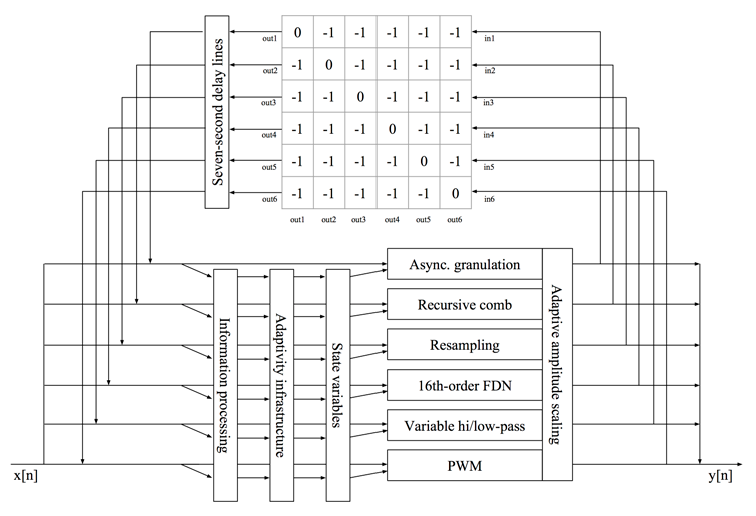
\includegraphics[width=14cm]{figures/OFNnetwork.pdf}
    \caption{Schema della rete di Order From Noise}
    \end{center}
\end{figure}

A parte le unità di elaborazione del suono,
in questo sistema,l'\textit{Information Processing} utilizzato per generare i 
segnali di controllo è diverso
dalle implementazioni tipiche riportate precedentemente nel corso di questa tesi;
piuttosto che calcolare \textit{feature extraction} come l'RMS, la diffusione spettale, ecc. 
Dario Sanfilippo utilizza in questo sistema una sorta di Low Frequency Oscillator
non lineare dipendente dal segnale in ingresso.
Questo comportamento viene ottenuto utilizzando un filtro Lowpass per far 
passare solo le componenti energetiche di un segnale sotto la soglia di 1Hz,
come ad esempio segnali a 0,01Hz, il segnale risultante viene poi processato
tramite normalizzazione dinamica per essere riportato ad una soglia in ampiezza
in un range fra [-1; 1],
viene elevato a una potenza relativamente grande per forzarlo intorno a 0,
ed infine utilizzato per pilotare la frequenza di un fasore.\\

\vspace{0.5cm} 
\lstinputlisting[breaklines, frame=trBL, caption={non linearità in Order From Noise}]
{codes/OFNnonLinearity.dsp}

La funzione \verb|lowFreqNoise(x)| accetta un segnale in ingresso
facendolo passare per uno stadio di 4 filtri Lowpass a cascata,
dove la stessa frequenza di taglio viene passata esternamente 
dalla variabile \verb|refPeriod|.
Il segnale passa poi per il normalizzatore dinamico composto dalle funzioni
\verb|noiseRMS(x)| e \verb|normRMS(x)|,
questo tipo di normalizzazione dinamica si basa sulla stima RMS e ha due ingressi,
uno è il segnale di riferimento, e l'altro è il segnale che deve essere normalizzato sulla base
del segnale di riferimento fornito, ovviamente,
la finestra RMS deve essere abbastanza grande a seconda della lentezza del
segnale che deve essere normalizzato.\\ 
Per comprendere meglio i meccanismi alla base
della normalizzazione dinamica,
andrò a discutere ora il caso più generico
di una normalizzazione di picco in DSP. \\
Partendo dall'algoritmo basilare del \textit{Peakholder} in IIR discusso nel precedente capitolo. 
L'ampiezza del picco di un segnale può essere normalizzata secondo la seguente espressione 

\begin{align*}
    y_{1}(t) = (1/(\max\left( y_{1}(t\!-\!1), \left\lvert{x(t)}\right\rvert \right))) * x(t) 
\end{align*}

dove \textit{x} è il segnale in ingresso, e \textit{y} il segnale sia in uscita che reiterato nella funzione. \\
Per prima cosa si calcola con il \textit{Peakholder} il picco massimo del segnale,
tracciandone il profilo di ampiezza campione per campione,
e a seguito si divide poi il risultato per 
un fattore per cui si desidera riscalare il segnale, in questo caso una costante 1.
Ed infine il profilo di ampiezza risultante da questa operazione verrà moltiplicato 
per lo stesso segnale in ingresso, incrementando o riducendo l'ampiezza di questo in base al risultato dell'operazione, 
e ridimensionando grazie a questo processo l'ampiezza di tutti i campioni del segnale, 
in modo tale che l'ampiezza del picco abbia un valore pari a [1, -1].

\vspace{0.5cm} 
\lstinputlisting[breaklines, frame=trBL, caption={Algoritmo di normalizzazione di picco tramite \textit{Peakholder} ad 1 campione di ritardo}]
{codes/PeakNormalizationIIR.dsp}

\begin{figure}[h!]
\begin{center}
    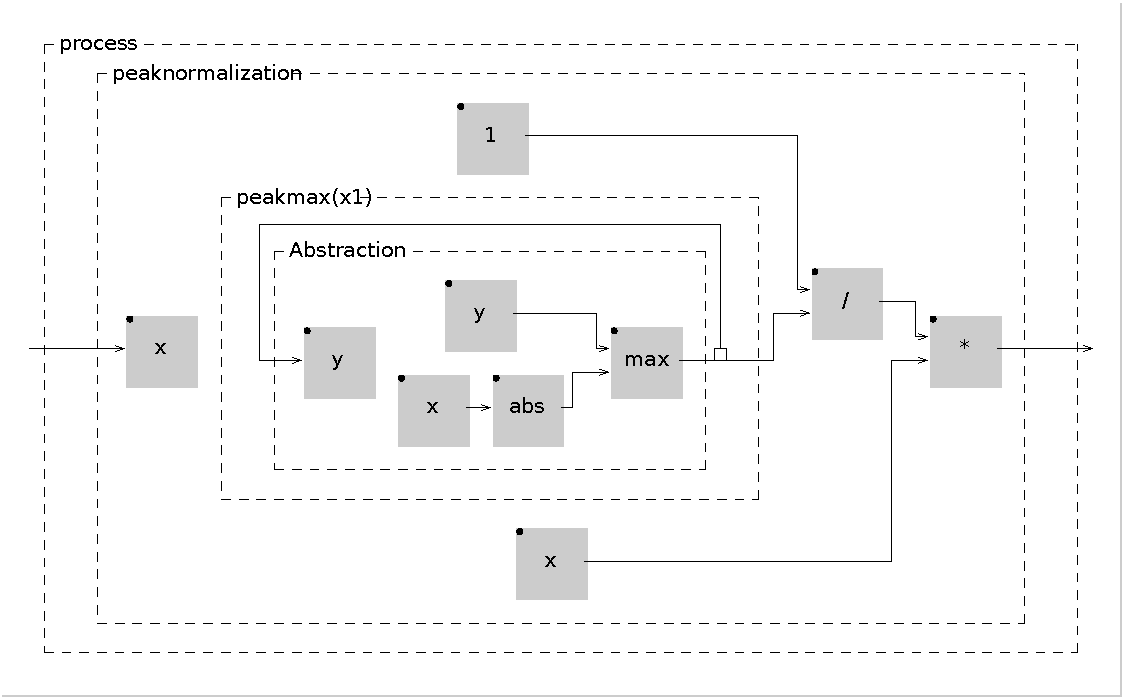
\includegraphics[width=14cm]{figures/PeakNormalizationIIR.pdf}
    \caption {Topologia del normalizzatore di picco tramite \textit{Peakholder} ad 1 campione di ritardo}
\end{center}
\vspace{0.5cm}
\end{figure}
    
Proprio come nell'algoritmo del \textit{Peakholder} ad 1 campione di ritardo, 
il problema di questa applicazione dipende dal fatto che nel segnale
complessivo possano permanere contributi spuri che alterino il risultato
della normalizzazione, e che si possa generare aliasing a causa di una mancata
funzione di smoothing del segnale.
Per questi motivi nelle unità della rete di Order From Noise 
che implementano al proprio interno meccanismi di Feedback,
e per raggiungere quindi una stabilità globale della rete,
è presente un tipo di limiter dinamico chiamato da Dario Sanfilippo
col nome di \textit{Lookahead Limiter}, che a differenza dell'algoritmo
appena discusso ha un comportamento adattivo.
Questo tipo di Algoritmo viene descritto da Dario Sanfilippo sia nell'articolo 
di Musica/Tecnologia dell' 11-12 (2017-2018) che parla di Order From Noise 
citato precedentemente,\footcite{sanfilippo_time-variant_2018}
che nel suo blog, dove ne riporta un implementazione fatta nel linguaggio di programmazione
Pure Data.

\begin{center}
    \vspace{0.5cm}
    \textit{Recently, I have decided to try the design of a limiter based on a post by IOhannes Zmölnig who, 
    in turn, has based his design on the thesis project by Peter Falkner: 
    Entwicklung eines digitalen Stereo-Limiters mit Hilfe des Signalprozessors DSP56001.
    This design is based on a peak-hold module with an exponential decay curve...
    The first step in a lookahead limiter is to delay the input signal so 
    that the attenuating curve can anticipate fast peaks. 
    The amplitude profile of the input signal is obtained by combining a peak-hold module 
    – something that holds a peak for a certain time until a new peak is detected – 
    with a peak envelope one to have a smooth decay when signals transition to lower peaks. 
    Here, after, the peak-hold module, 
    I am also using a one-pole low-pass filter with a period matching that of the input delay 
    so that peaks and input signal are synchronised and the attack is slightly smoothed out... 
    The peak envelope can easily be implemented as a single feedback loop through which the detected peaks recirculate}\\
    \vspace{0.5cm}
    Lookahead limiting in Pure Data - July 2, 2017
    \footcite{https://www.dariosanfilippo.com/blog/2017/lookahead-limiting-in-pure-data/}
    \vspace{0.5cm}
    \end{center}

Per implementare il \textit{Lookahead Limiter} 
sono dunque richieste due unità distinte
combinate fra loro in Feedforward con un filtro onepole Lowpass fra le due,
un \textit{Peakholder} con una finestra che mantiene il picco massimo del segnale e
che viene resettata da un timer, 
e un \textit{Peakenvelope} che ha invece un decadimento 
basato su \textit{tau} all'interno della retroazione; sono entrambe due
unità ottimizzate del nostro algoritmo \textit{Peakholder} ad 1 campione di ritardo,
e che combinate fra loro consentono di rilevare sia i transienti di attacco rapidi, 
che al contempo di avere una lunga fase di decadimento per i suoni sostenuti e lenti.\\
Il \textit{Peakenvelope} può essere ottenuto modificando 
la retroazione dell'algoritmo \textit{Peakholder}, moltiplicandola per 
un fattore di decadimento come nella seguente formula 

\begin{align*}
    y_{1}(t) = \max\left( k_{1} * y_{1}(t\!-\!1), \left\lvert{x(t)}\right\rvert \right)
\end{align*}
dove 
\begin{align*}
    k_{1} = {0.001}^{\frac{T}{ST}} 
\end{align*} 

è la formula del decadimento RT60, 
e dove \textit{T} rappresenta il tempo di decadimento desiderato in secondi, 
mentre \textit{ST} rappresenta la durata di un campione in secondi per la frequenza di campionamento corrente.
Come nelle altre formule del \textit{Peakholder}, \textit{x} è il segnale in ingresso, 
e \textit{y} il segnale sia in uscita che reiterato nella funzione stessa. \\
A seguito l'algoritmo in Faust del \textit{Peakenvelope}.

\vspace{0.5cm} 
\lstinputlisting[breaklines, frame=trBL, caption={Algoritmo di \textit{Peakenvelope} con Decay RT60}]
{codes/PeakEnvelope.dsp}

\begin{figure}[h!]
\begin{center}
    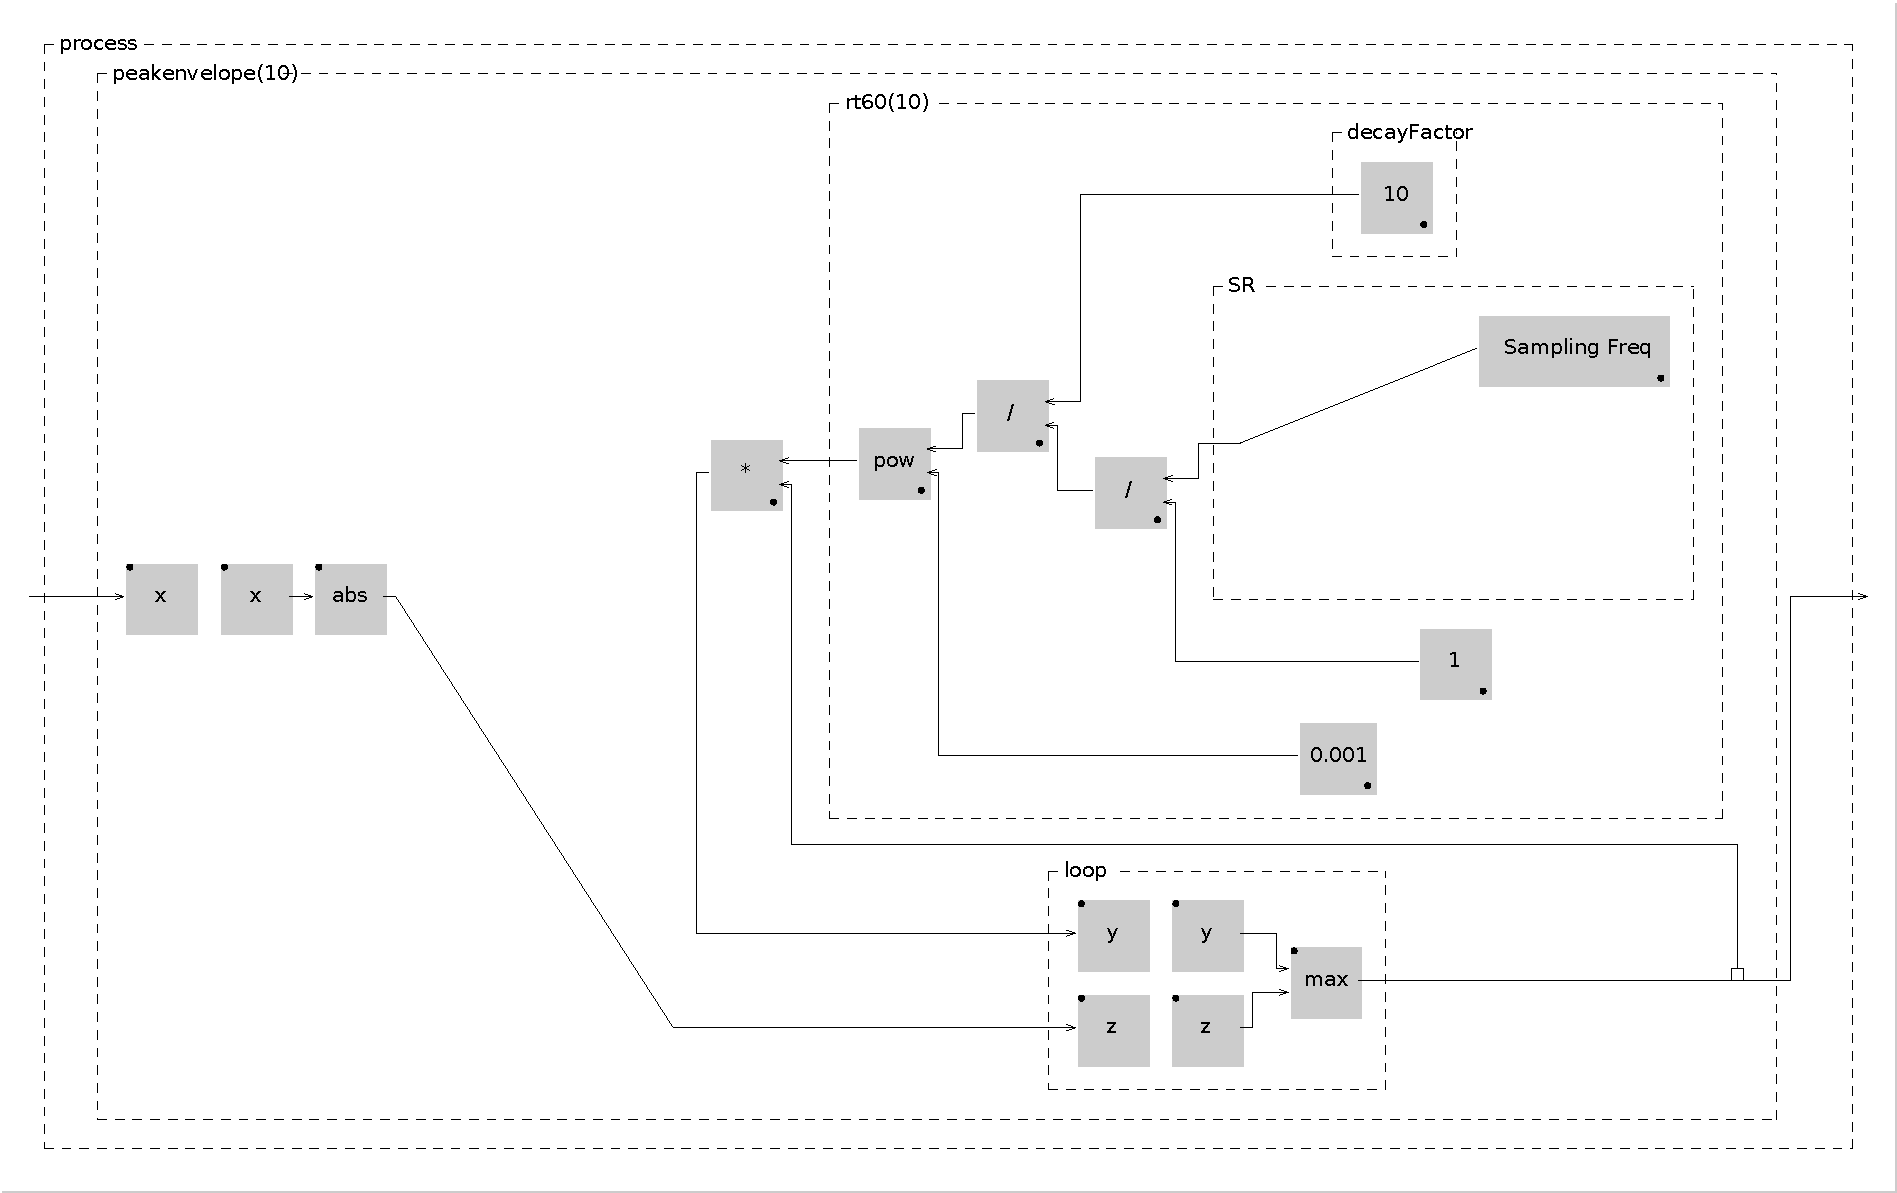
\includegraphics[width=15cm]{figures/PeakEnvelope.pdf}
    \caption{Topologia del \textit{Peakenvelope} con Decay RT60}
\end{center}
\vspace{0.5cm}
\end{figure}

per quanto riguarda invece l'algoritmo del \textit{Peakholder} adattivo, è un po' meno semplice. 
Il \textit{Peakholder} verificherà se l'ingresso è maggiore o uguale all'uscita e, 
se la condizione è vera, aggiornerà il picco e ripristinerà un timer. 
Quando la condizione invece è falsa, 
inizierà il suo countdown e, allo scadere del tempo, se non è stato rilevato alcun nuovo picco, 
qualsiasi valore nell'ingresso corrente verrà impostato come nuovo picco.

\vspace{0.5cm} 
\lstinputlisting[breaklines, frame=trBL, caption={Algoritmo del \textit{Peakholder} (adattivo) con Timer}]
{codes/PeakHolderAdaptive.dsp}
\clearpage

\begin{figure}[h!]
\begin{center}
    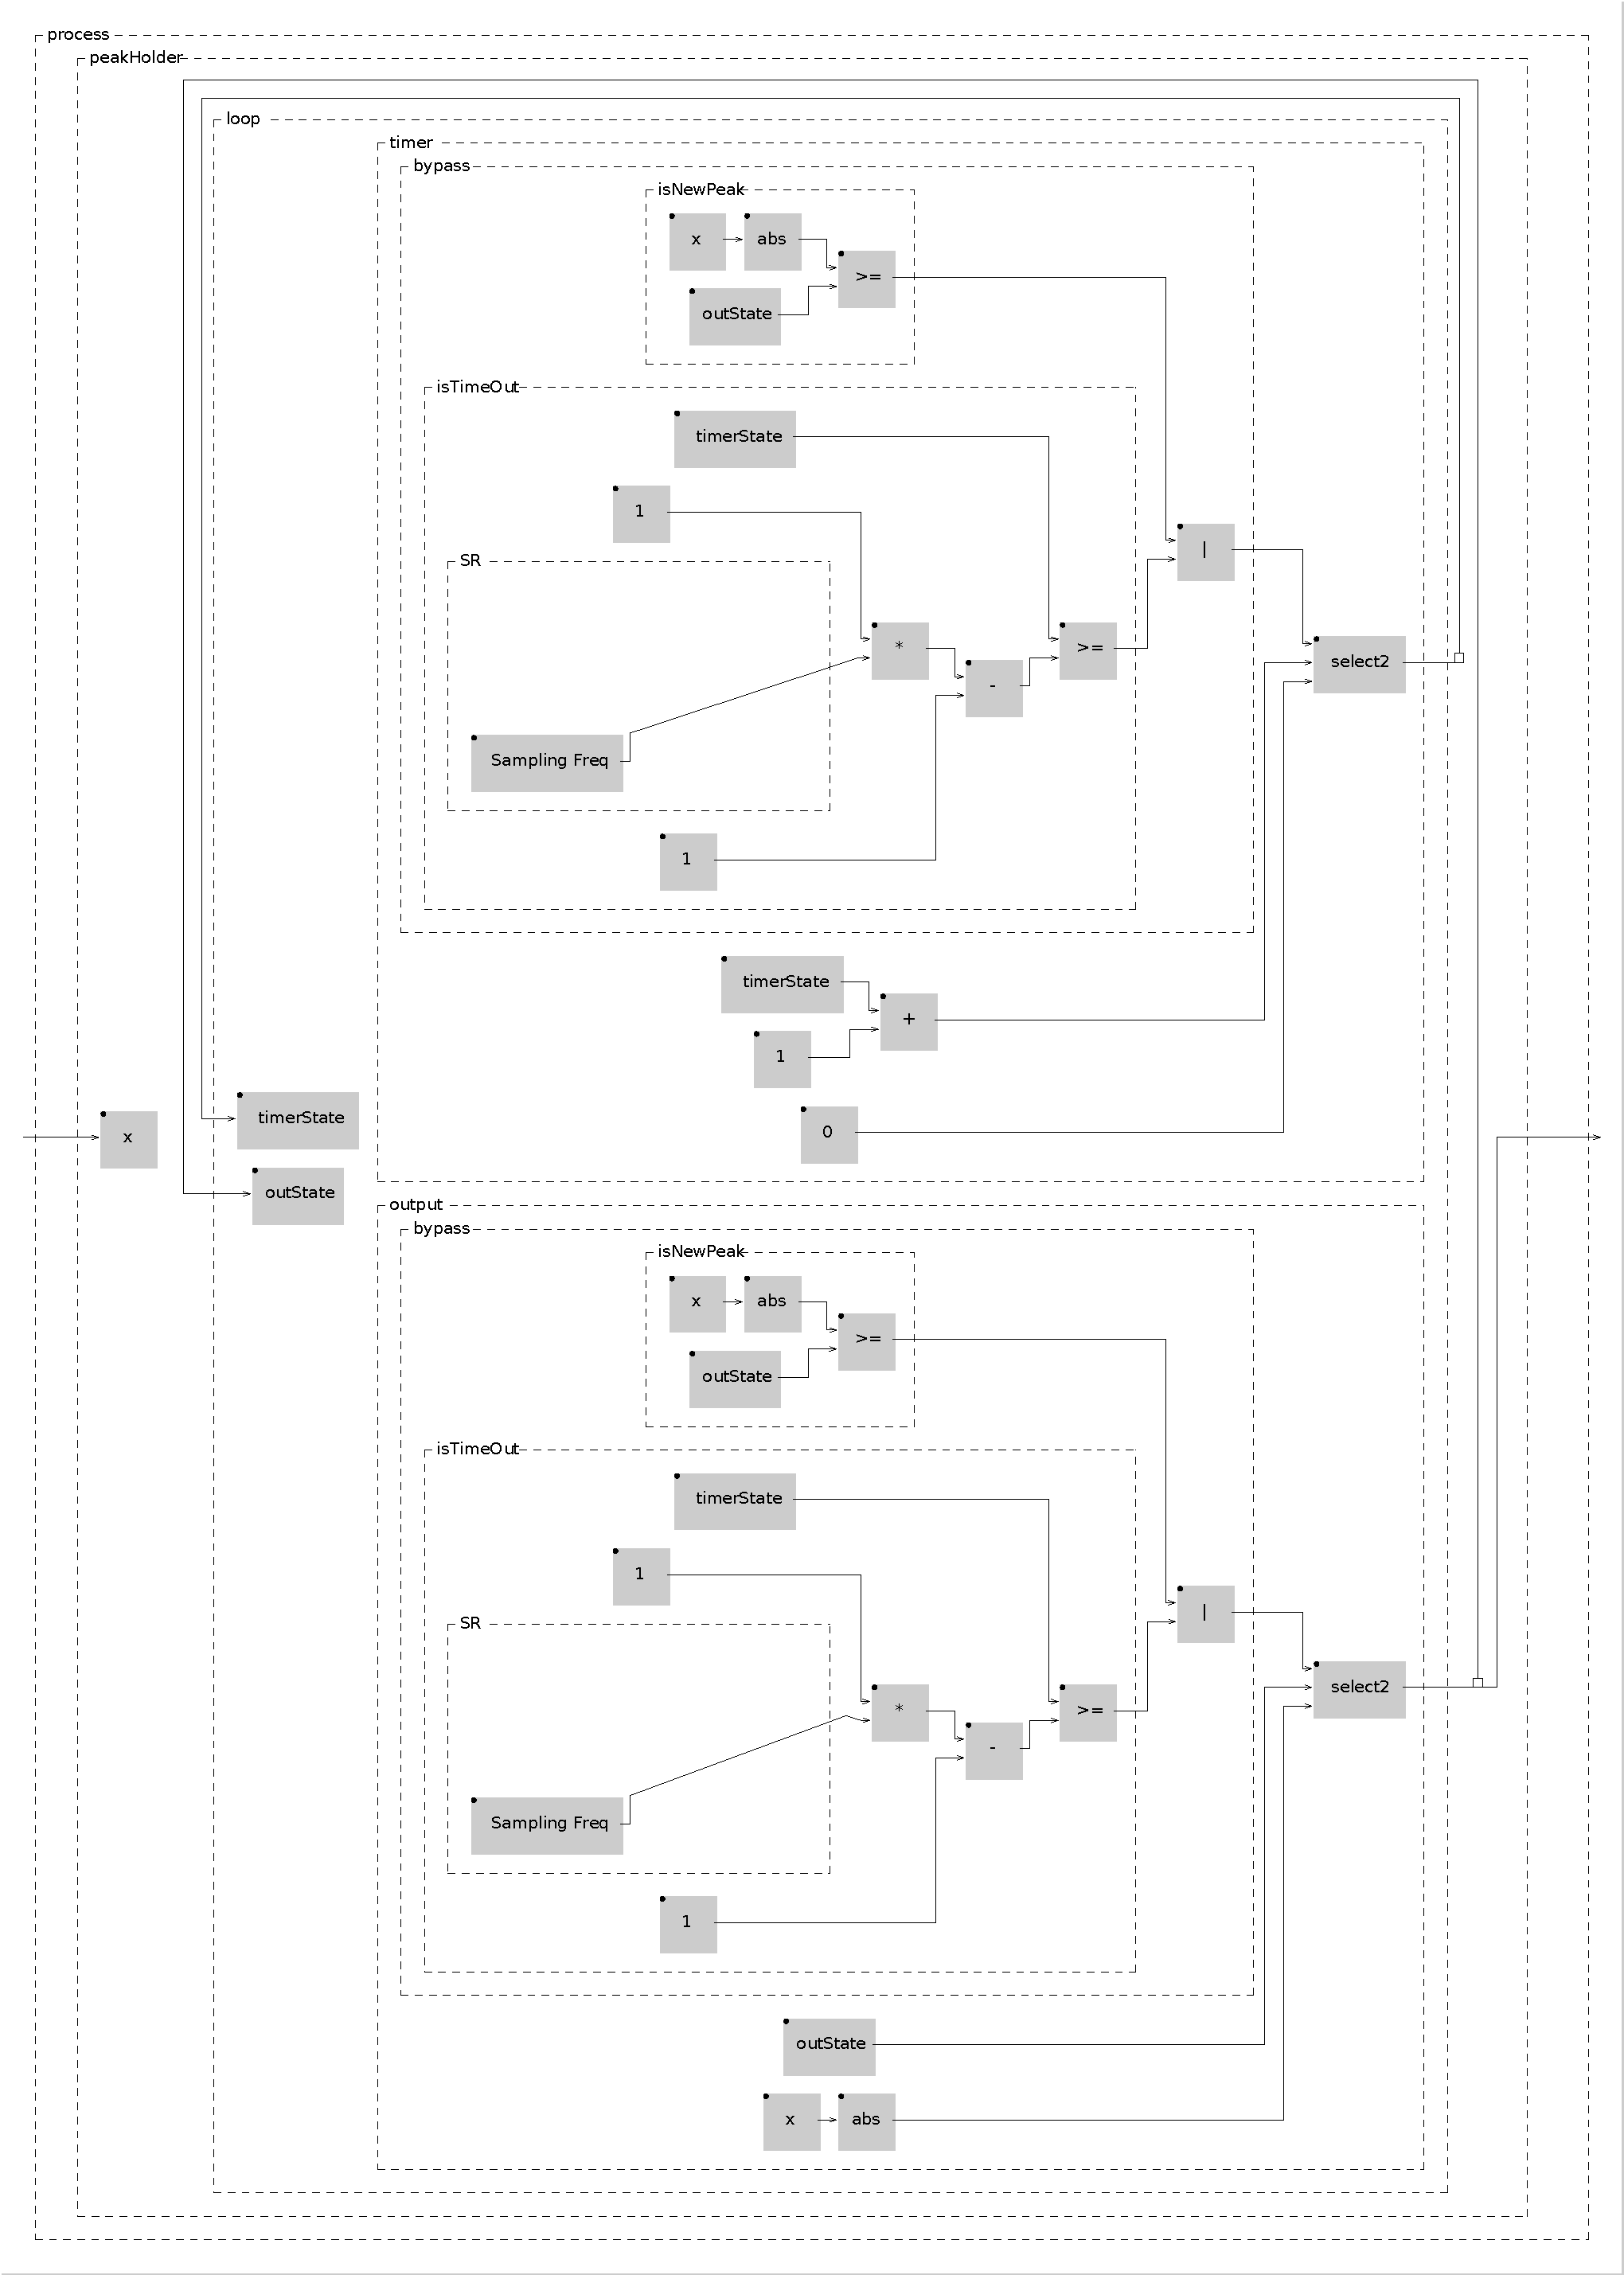
\includegraphics[width=15cm]{figures/PeakHolderAdaptive.pdf}
    \caption{Topologia del \textit{Peakholder} (adattivo) con Timer}
\end{center}
\vspace{0.5cm}
\end{figure}
\clearpage

Per concludere infine le unità sono combinate fra loro come a seguito,
formando nel loro insieme il \textit{Lookahead Limiter}.

\vspace{0.5cm} 
\lstinputlisting[breaklines, frame=trBL, caption={Algoritmo del \textit{Lookahead Limiter}}]
{codes/LookaheadLimiter.dsp}

Prima di concludere queste considerazioni a seguito qualche doverosa aggiunta.
Anche nell'Ecosistemico Udibile n.2, studio sul Feedback, di Agostino Di Scipio è presente 
una versione ottimizzata dell'algoritmo \textit{Peakholder}, che a differenza
del \textit{Peakholder} con il timer discusso precedentemente, viene chiamato come
\textit{Local Max}, e riporta l'ampiezza massima solamente al termine del \textit{time frame} che corrisponde
al reset del timer, senza necessità della complessa condizione vero/falso discussa precedentemente, 
ma a discapito di un tempo di ritardo dovuto all'analisi del valore massimo che viene riportato 
solo al termine del \textit{time frame}.
In partitura viene descritto come segue:

\begin{center}
    \vspace{0.5cm}
    \textit{local max = returns the maximum signal amplitude (absolute value) 
    in a given time frame; frame duration is dynamically adjusted: 
    the next frame duration is set at the end of the previous frame} \\
    \vspace{0.5cm}
\end{center}

A seguito l'implementazione del \textit{Local Max} in Faust.

\vspace{0.5cm} 
\lstinputlisting[breaklines, frame=trBL, caption={Algoritmo del \textit{Local Max}}]
{codes/LocalMax.dsp}

\subsection{Conclusioni}
\label{sec:Conclusioni}

In conclusione, abbiamo avuto modo di approfondire alcuni dei principali meccanismi 
utilizzati da Dario Sanfilippo nel suo brano Order From Noise \textit{(Homage to Heinz Von Foerster)},
prendendo questo lavoro come caso di studio, con il fine di illustrare
alcune modalità e relazioni possibili per rendere un sistema autonomo e 
capace di manifestare comportamenti emergenti e complessità anche all'interno di uno 
spazio deterministico interamente costituito solo dal DSP nel software 
(che abbiamo chiamato qui col nome di spazio latente); 
inclusi metodi e strategie per la generazione delle relative non linearità,
e meccanismi adattivi per mantenere il sistema in una condizione di stabilità
controllata tramite algoritmi di Feedback positivo e negativo.
Anche qui i meccanismi contenuti all'interno del brano ovviamente non si limitano solamente a questi,
ma si è cercato di approfondire le parti del sistema che riguardano l'\textit{Audio Information Processing};
così da fornire strumenti che rendono possibile affrontare il problema 
dell'adattattività e dell'\textit{adattattività dinamica}
all'interno dei CASes, lasciando comunque aperta la possibilità di poter approfondire il brano a partire
dai testi citati in bibliografia, che riportano anche le formule matematiche e la descrizione
per gli altri moduli e le altre unità del brano brano.

\clearpage

\thispagestyle{empty}
%!TEX encoding = UTF-8 Unicode
%!TEX root = ../thesisCASes.tex

%% TITOLO
\section{Sistemi Caotici}
\label{sec:Sistemi Caotici}

Ciò che accomuna un sistema complesso ad un sistema caotico è la non linearità.
In questa visione della complessità, i sistemi caotici sono considerati un sottoinsieme 
appartenente alla macrocategoria dei sistemi complessi: la complessità 
si manifesta infatti sulla soglia della caos. 
Mentre nel mondo fisico la non linearità è insita nella natura
delle cose, nel mondo digitale, queste non linearità, come abbiamo visto
anche nei capitoli precedenti, devono essere accuratamente
programmate ed introdotte all’interno degli algoritmi per raggiungere la complessità. \\
La teoria del caos postula che esista una classe di fenomeni naturali che
possano essere modellati da sistemi deterministici non lineari.
Quando si parla di caos ci si riferisce ad un certo tipo di comportamento di
un sistema dinamico: determinato dalla sensibilità alle condizioni iniziali,
imprevedibilità a lungo termine, e orbite periodiche dense. \\ 
In altri termini un sistema caotico amplifica le piccole differenze: porta i fenomeni microscopici
a un livello macroscopico. Ed è dunque nell’amplificazione di queste piccole
deviazioni delle condizioni iniziali che si annida il caso.
Nonostante siano perfettamente individuate le equazioni differenziali che
descrivono questi sistemi: al variare delle condizioni iniziali 
varia il comportamento del sistema stesso negli stadi successivi a quello iniziale.
L’ipotesi che i sistemi deterministici possano sviluppare comportamenti impredicibili, 
come già detto all'inizio di questa tesi fu teorizzata da Henri Poincaré e portata alla
fama da Edward Norton Lorenz con il suo articolo.\footcite{Lorenzdnf}
In questo capitolo della tesi, illustrerò attraverso la composizione di un mio brano, 
come a partire dalla risoluzione delle equazioni differenziali del sistema di Lorenz, si possa
creare un CAS che possa essere utilizzato per la
performance musicale in live electronics.

\subsection{RITI : Room Is The Instrument}
\label{RITI : Room Is The Instrument}

RITI: Room Is The Instrument è un brano che si basa su un Sistema Complesso \textit{site-specific},
in grado di manifestare comportamenti emergenti e caotici,
dove la personalità acustica della stanza in cui viene eseguito il brano può
essere riflessa in variazioni del comportamento del sistema stesso.
L'idea dell'acronimo RITI deriva dal famoso paper di Agostino Di Scipio 
"Sound is the interface" (SITI), 
che ha introdotto per la prima volta la prospettiva sistemica 
sull'auto-organizzazione e sulla capacità di un sistema di auto-osservarsi 
tramite l'ambiente circostante in musica.\footcite{di_scipio_sound_2003} \\
Il sistema è costruito utilizzando alla base una soluzione 
delle equazioni differenziali del sistema di Lorenz come motore di sintesi del suono in DSP;
Le esigenze di questo tipo di applicazioni nel mondo della Computer Music
sono generalmente motivate dal desiderio di esplorare i comportamenti complessi ed emergenti
che questo tipo di sistemi manifesta.
Il modello delle Equazioni di Lorenz che ho seguito per questo tipo di sistema, si basa
su delle costrizioni matematiche aggiunte alle risoluzioni
per esplorare il sistema in regioni instabili, 
seguendo il metodo descritto nel paper di Dario Sanfilippo 
"Constrained Differential Equations as Complex Sound Generators".\footcite{sanfilippo_constrained_2021} 
Dove vengono illustrate una serie di risoluzioni per alcune 
equazioni differenziali caotiche,
modificate inserendo opportunamente all'interno di queste un
DC Blocker e un Waveshaper (soft clipping) utilizzando la funzione della tangente iperbolica.
Oltre alle costrizioni proposte da Dario Sanfilippo, 
ispirato dall'idea che ha avuto Tom Mudd nel suo paper
"Between Chaotic Synthesis and Physical Modelling: Instrumentalising with Gutter Synthesis",\footcite{tom_mudd_gutter_synthesis}
di aggiungere alla risoluzione dell'equazione differenziale dell'Oscillatore di Duffing
un banco di filtri Bandpass che permettesse al sistema di manifestare
risonanze modali che ricordino il comportamento di uno strumento musicale.
Ho deciso di aggiungere alla risoluzione delle equazioni di Lorenz modificate,
un banco parallelo di 32 filtri Bandpass informati 
con 4 liste ricavate dall'analisi di 4 registrazioni di note diverse di un violoncello, 
per ottenere una complessità costretta dalle risonanze modali di questi filtri.
Per concludere, ho aggiunto infine alle tre equazioni l'ingresso di un segnale esterno, 
affidato ai microfoni, 
che permettesse di perturbare il sistema e generare un ulteriore stato 
di feedback proveniente dall'ambiente della performance,
rendendo così il sistema di sintesi sensibile alle condizioni esterne.
L'equazione di Lorenz modificata con le costrizioni esposte,
costituisce nel suo insieme un singolo agente, a cui ci riferiremo a partire da questo
momento con il nome di CSGA \textit{Complex Sound Generator Agent}, e che verrà richiamato a seguito
all'interno di una superiore \textit{Feedback Delay Network} (FDN) che ne contiene un 
numero finito voci determinato a tempo di compilazione. 
Prima della performance, in fase di compilazione del sistema,
è quindi possibile scegliere il numero di CSGA che andranno a costituire 
la FDN, e di conseguenza il numero di altoparlanti da utilizzare
per ascoltare l'output da ogni agente della rete.
Tuttavia, si può anche decidere di ascoltare solo un certo numero di output
della rete a partire da un numero di altoparlanti ridotti nello spazio della performance,
senza rinunciare alla complessità derivata da una compilazione con un
numero di agenti che costituisce la rete superiore al numero di ouput che si vogliono ascoltare, 
ad esempio: 16 CSGA che costituiscono la rete ma ascoltandone solo 4 dagli Altoparlanti.
Il feedback globale della rete proveniene da ogni singola voce 
che va a sommarsi con diversi tempi di ritardo prima della retroiniezione,
rientrando poi conseguentemente con opportuni tempi di ritardo nelle altre voci del sistema.
Questo processo crea una decorrelazione ed una perturbazione nei singoli agenti all'interno del sistema,
ma offre anche la possibilità con opportuni valori di Gain del feedback della FDN, 
di lasciar ricirolare del materiale nella rete.
La performance consiste nell'impostare un insieme iniziale di valori 
di inizializzazione del sistema, come Dt, Rho, Beta, Sigma, 
tangente iperbolica, 
un fattore di Shift in frequenza del banco di filtri, 
Tempi di ritardo della FDN, ecc.
E a partire da questi, l'obiettivo è di esplorare il sistema 
finché non si ha l'impressione di aver esaurito tutte le possibilità, 
con l'obiettivo fondamentale di bilanciare i tre feedback principali: 
quelli provenienti dalle retroazioni delle tre equazioni differenziali 
di Lorenz, quello della FDN, e quello proveniente dal contributo 
dell'ambiente di performance.
Nelle sezioni successive della tesi, 
discuteremo in dettaglio tutti questi aspetti passo per passo
come fatto fino ad ora con i lavori precedenti. 

\subsection{Complex Sound Generator}
\label{Complex Sound Generators}

La nozione di Complex Sound Generator è stata ripresa qui a partire dal
paper di Dario Sanfilippo\footcite{sanfilippo_constrained_2021},
tuttavia nella letteratura della Computer Music, primi esempi di applicazioni
di sistemi caotici per la generazione di suoni nella musica risalgono
ai primi anni '90 con gli esempi portati da Agostino Di Scipio
in suoi articoli come “Composition by exploration of non-linear dynamic systems”.\footcite{discipioiterated}
O nel corso degli anni '90 con gli studi di Lorenzo Seno al Centro Di Ricerche musicali
di Roma sui modelli fisici ed il Caos, con applicazioni nelle composizioni di Michelangelo Lupone.
Le radici della sintesi caotica in generale sono multiple e dipendono
dalla definizione del campo di applicazione, si potrebbe far risalire
a David Tudor con i suoi esperimenti cibernetici sul feedback elettrico del 1960
così come alle implementazioni specifiche esplorate da molti artisti
delle equazioni di Rössler nella sintesi video e audio.\footcite{tom_mudd_gutter_synthesis}
Il modello delle Equazioni utilizate alla base del CSGA si basa sul modello di Lorenz 
che fu il primo esempio di un sistema di equazioni differenziali a bassa
dimensionalità in grado di generare un comportamento caotico.
Venne scoperto da Edward N. Lorenz, del Massachusetts Institute of Technology, nel 1963.
Semplificando le equazioni del moto alle derivate parziali che descrivono il movimento termico di
convezione di un fluido, Lorenz ottenne un sistema di tre equazioni differenziali del primo ordine.
La versione continua dell’equazione differenziale che descrive il modello di Lorenz è descritta come segue: 

\begin{align*}
\frac{\partial x}{\partial t} & = \sigma(y-x) \\
\frac{\partial y}{\partial t} & = \rho x - xz - y \\
\frac{\partial z}{\partial t} & = xy -\beta z 
\end{align*}

Dove \( x \) è proporzionale all’ampiezza della circolazione della velocità del fluido nell’anello del fluido,
il positivo rappresenta il moto in senso orario ed il negativo il senso antiorario,
dove \( y \) è la differenza di temperatura tra i fluidi superiori ed inferiori,
e dove \( z \) è la distorsione dalla linearità del profilo della temperatura verticale.
Mentre \( \sigma,  \rho,  \beta \) governano la relazione fra le quantità (e sono maggiori di 0),
e \( \partial t \) rappresenta lo step d'integrazione. \\
Mentre per una sua rappresentazione in forma di modello discreto,
può essere scritto un algoritmo in Faust come segue:

\vspace{0.5cm} 
\lstinputlisting[breaklines, frame=trBL, caption={Algoritmo del Sistema di Lorenz Discreto}]
{codes/LorenzSystem.dsp}
\clearpage

\begin{figure}[h!]
\begin{center}
    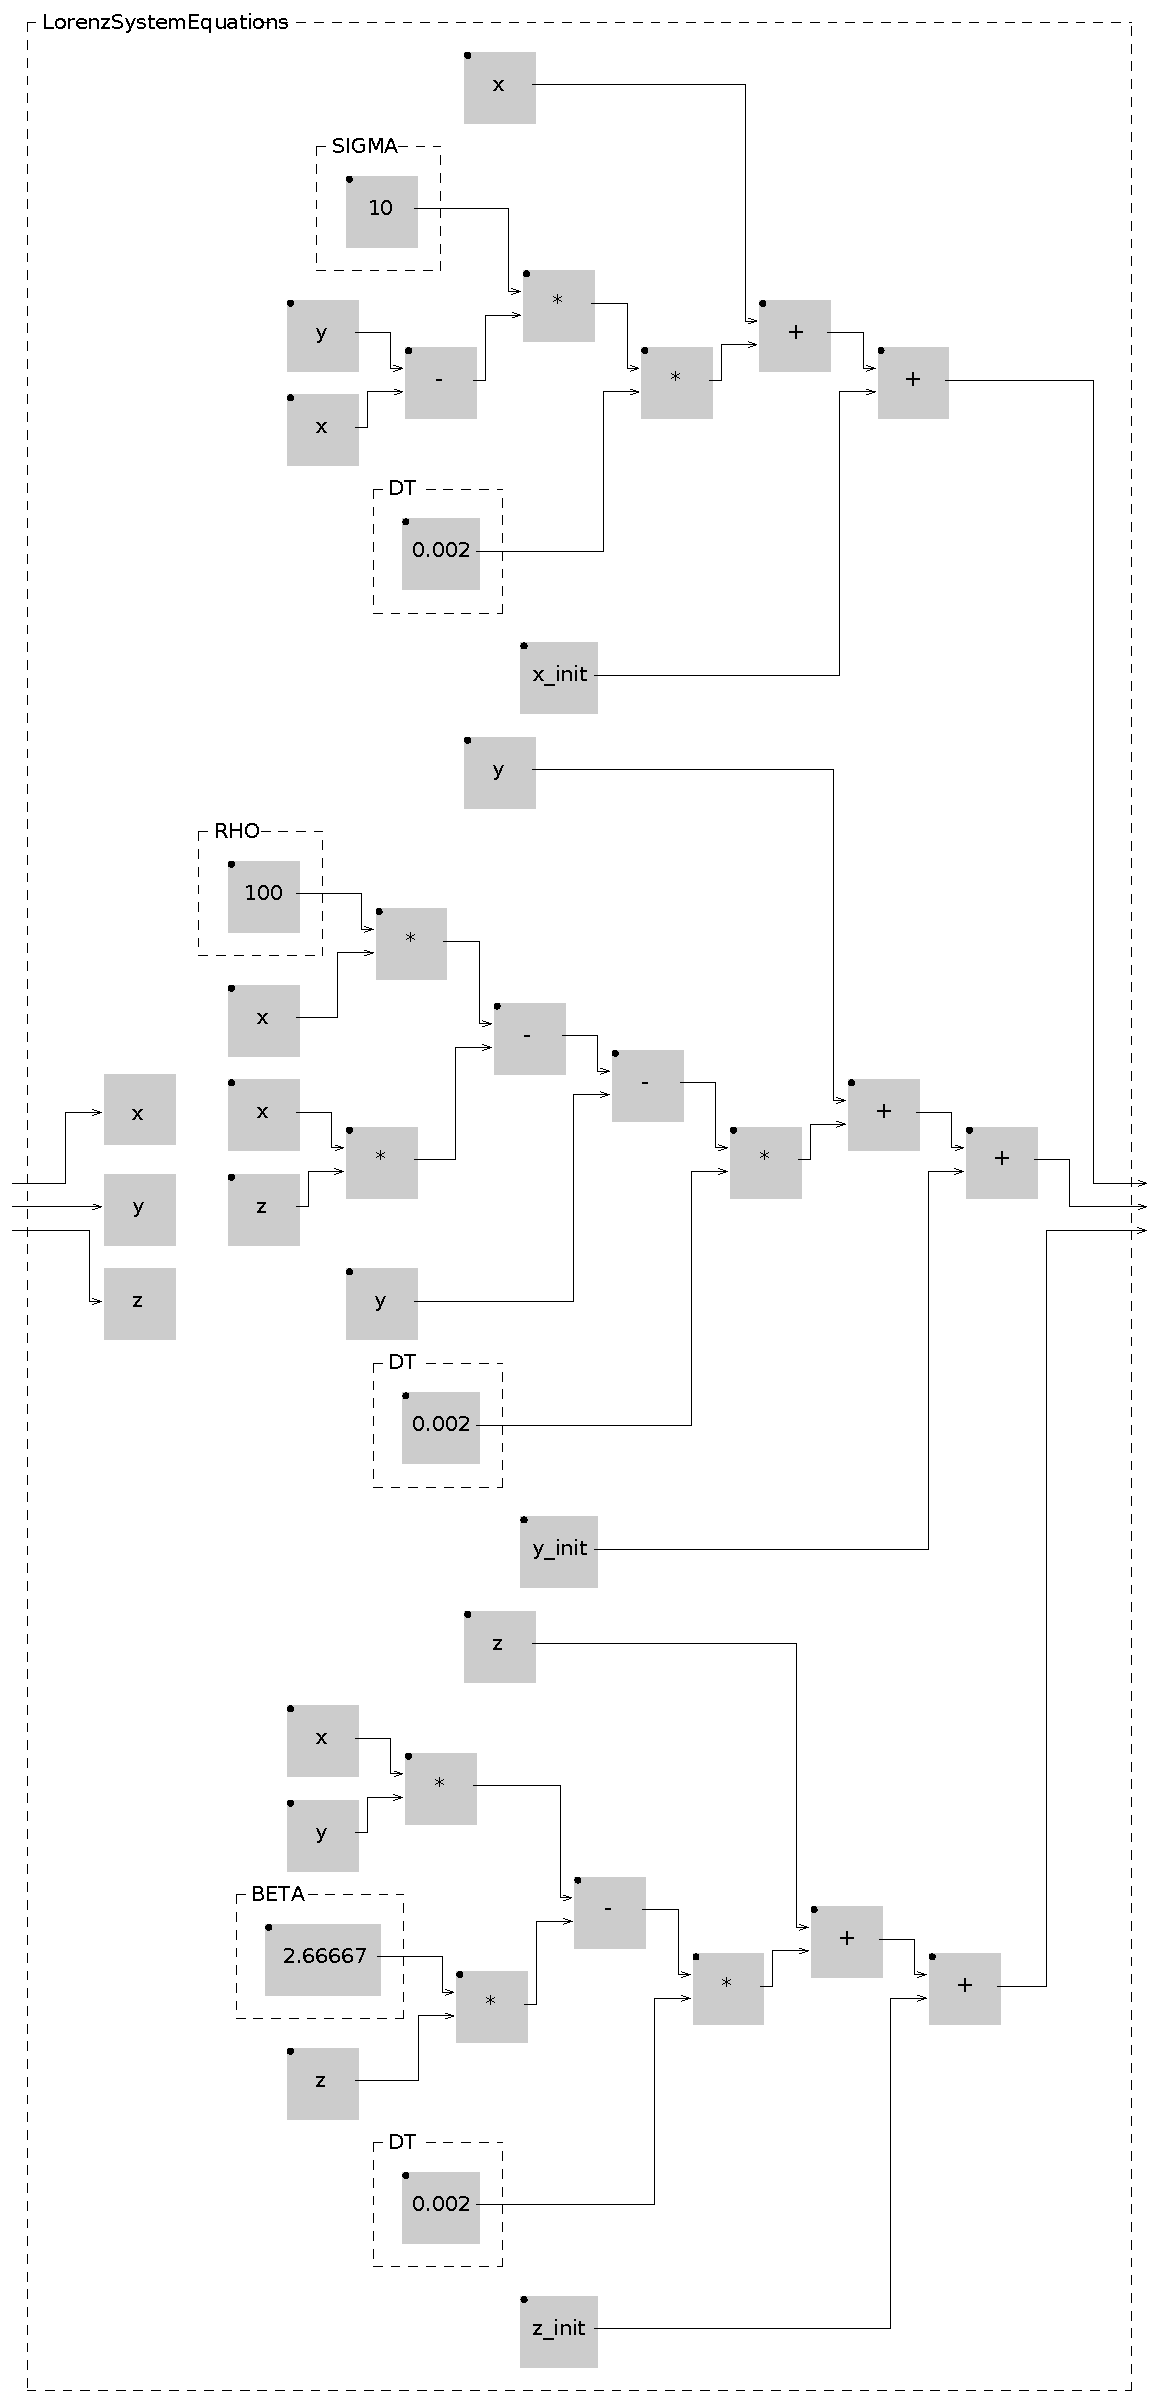
\includegraphics[width=11.5cm]{figures/LorenzSystemInside.pdf} 
    \caption{Topologia dell'Algoritmo del Sistema di Lorenz Discreto} 
\end{center}
\vspace{0.5cm}
\end{figure}
\clearpage

\begin{figure}[h!]
\begin{center}
    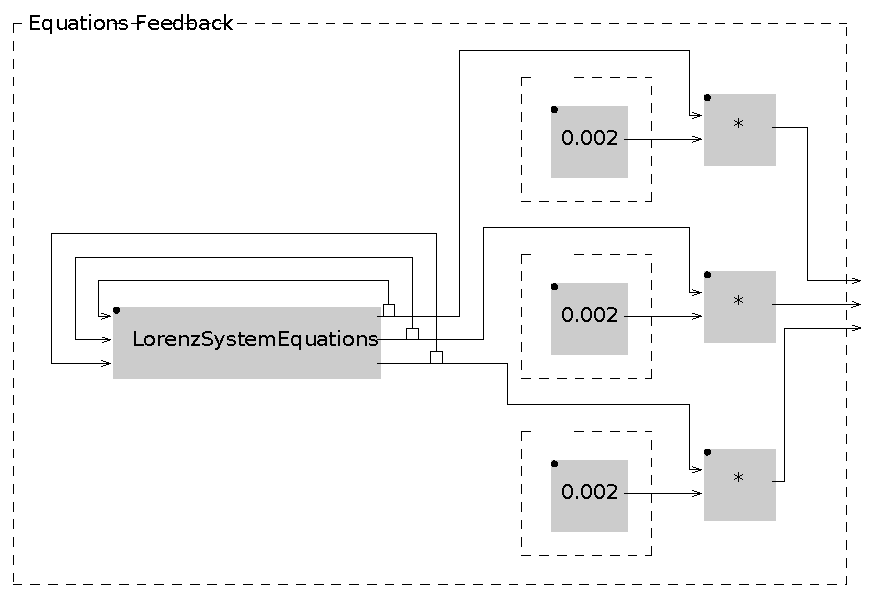
\includegraphics[width=14cm]{figures/LorenzSystemFB1.pdf}
    \caption{Topologia del Feedback delle Equazioni del Sistema di Lorenz Discreto}
\end{center}
\vspace{0.5cm}
\end{figure}

Questo algoritmo permette già di produrre sintesi attraverso la 
risoluzioni delle Equazioni del Sistema di Lorenz, ma per il momento in modo acritico.
Come detto in precedenza, esistono ricerche che si pongono il problema 
di un adattività dei sistemi caotici con il fine di poterli utilizzare per determinati scopi,
andrò adesso ad illustrare nel dettaglio i modelli che ho preso 
a riferimento in questo brano per poter utilizzare
i sistemi caotici per fini musicali di sintesi del segnale. \\
Per poter esplorare un sistema caotico con il fine di creare un segnale udibile in tutte le sue regioni, 
è necessario dunque porsi dunque un problema di ottimizzazione;
è necessario chiedersi quali problemi possano verficarsi e quali strumenti possano contrastarli. 
I problemi nell'utilizzare Lorenz come segnale di sintesi 
sono in sostanza Il DC Offset, e i valori più grandi del range [1, -1].
Riguardo le soluzioni sappiamo che il DC blocker, 
è uno strumento indispensabile nella modellazione della guida d’onda
digitale e in altre applicazioni, e che può rimuovere la componente Continua del segnale 
che circola in una linea di ritardo. Questo consiste sostanzialmente in
un filtro FIR highpass, poiché le correnti continue possono essere viste come frequenze a
0Hz, ed infine un onepole in serie che recupera parte della cancellazione del FIR.
Mentre per la funzione della tangente iperbolica, sappiamo che è una funzione
non lineare appartenente alle funzioni iperboliche, che costituiscono una famiglia di funzioni 
elementari dotate di alcune proprietà analoghe e corrispondenti alle
proprietà delle ordinarie funzioni trigonometriche.
utilizzando la tangente iperbolica come un Waveshaper (soft clipping) possiamo 
esplorare il sistema caotico in tutte le sue regioni rimanendo sempre in un range [1, -1].
A tal proposito Dario Sanfilippo propone:\footcite{sanfilippo_constrained_2021}

\begin{center}
    \vspace{0.5cm}
    \textit{Considering first-order differential equations, 
we can obtain a generalisation of the modified systems discussed
here. Let \( y \) be a vector of functions, let \( x \) be an input vec-
tor, let \( F \) be a vector of functions of \( y \) and \( x \) ; let  \( C \) be
a vector of constraining functions. Written in differential
form with respect to time, we have that:}
\begin{center}
\begin{align*}
    \frac{\partial y(t)}{\partial t} & = C(F(x(t), y(t))) && \text{where} && C(z) = B(l * S(z(l)))
\end{align*}
\end{center}
    \textit{with B and S being, respectively, vectors of first-order
    DC-blockers and saturating nonlinearities with arbitrary
    saturation threshold piloted by the parameter l. The saturation threshold 
    becomes a key parameter for the interaction with the oscillators, while the overall output can be
    normalised to unity peak amplitudes for digital audio by
    merely dividing by l. While several types of bounded saturators are available, here, 
    we will focus on the well known 
    hyperbolic tangent function. Note that the input
    vector can be used to set the system’s initial conditions or
    as continuous perturbation through signals. In fact, these
    systems can also be deployed as nonlinear distortion units
    when operating under non-self-oscillating conditions.}
    \vspace{0.5cm}
\end{center}

Secondo il metodo appena esposto, le costrizioni possono essere rappresentate come

\begin{align*}
    \text{where B} && y(n) = x(n) -x(n-1) +Ry(n-1) \\
    \text{where S} && y(t) = tanh(x(t))
\end{align*}

Mentre per la rappresentazione di Lorenz in forma di modello discreto modificato,
può essere scritto un algoritmo in Faust come segue:

\vspace{0.5cm} 
\lstinputlisting[breaklines, frame=trBL, caption={Algoritmo del Sistema di Lorenz Modificato con DC-blocker e TanH}]
{codes/CostrainedLorenzSystem.dsp}

\begin{figure}[h!]
\begin{center}
    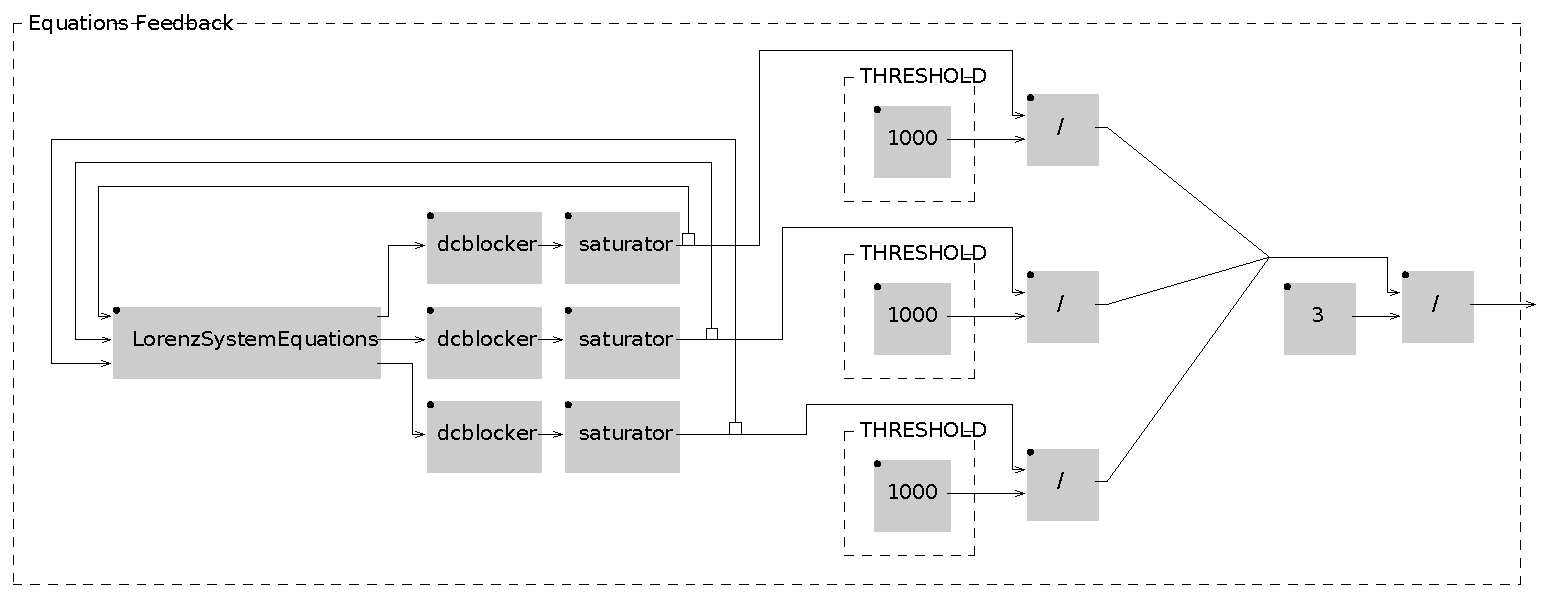
\includegraphics[width=14cm]{figures/LorenzSystemFB2.pdf}
    \caption{Topologia del feedback delle Equazioni del Sistema di Lorenz Modificato con DC-blocker e TanH}  
\end{center}
\vspace{0.5cm}
\end{figure}

\begin{figure}[h!] 
\begin{center}
    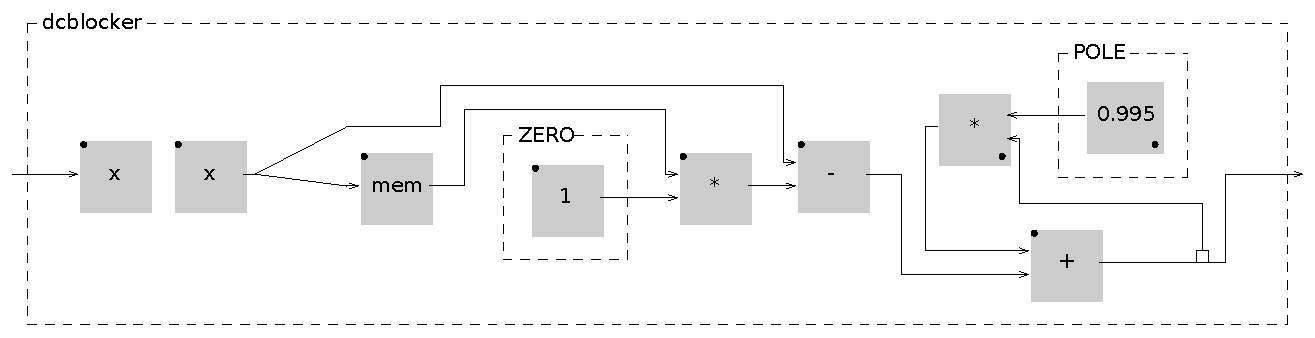
\includegraphics[width=14cm]{figures/DCblocker.pdf}
    \caption{Topologia dell'Algoritmo DC-blocker} 
\end{center}
\vspace{0.5cm}
\end{figure}
\clearpage

\begin{figure}[h!] 
\begin{center}
    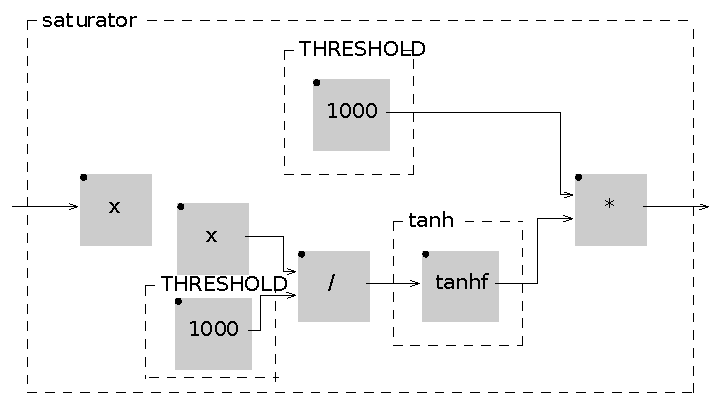
\includegraphics[width=10cm]{figures/Saturator.pdf}
    \caption{Topologia dell'Algoritmo TanH} 
\end{center}
\vspace{0.5cm}
\end{figure}

Ora il sistema di Lorenz è invece ottimizzato per la sintesi sonora.
Per concludere, il sistema di Lorenz Modificato passa infine per la sua terza costrizione,
che consiste in un Banco di Filtri Bandpass dove per un solo termine in ingresso 
il segnale viene diviso per il numero di banchi di filtri e restituito in uscita. \\
Il banco di filtri Bandpass è costituito da 32 voci parallele informate da 
4 liste di ricavate da analisi di 4 file audio di note del violocello,
esplorate durante il corso della performance.
L'algoritmo dei filtri Bandpass utilizzato come costrizione per il sistema
di Lorenz Modificato, consiste in un implementazione \textit{Virtual Analog} 
di un filtro del 2° ordine basato sulla struttura SVF \textit{State Variable Filter}.
La particolarità di questo tipo d'implementazione di SVF che ho utilizzato,
è che preserva matematicamente la topologia del filtro analogico,
includendo nella maggiorparte dei casi \textit{zero-delay loops}.
Questi filtri sono chiamati \textit{Topology Preserving Transform filters} o filtri TPT,
e provengono dal libro "The Art of VA Filter Design" di Vadim Zavalishin,\footcite{Zavalishin_VA_filter_design}
pubblicato e reperibile gratuitamente in rete. \\
A seguito riporto l'implementazione matematica di questo filtro SVF TPT di Vadim Zavalishin
che ha esposto Will Pirkle in un suo articolo chiamato 
"Virtual Analog (VA) Filter Implementation and Comparisons v2.0"\footcite{Pirkle_VA_filter_design}
del 2013 e reperibile dal suo sito.

\begin{align*}
    y_{hp}(n) = & \frac{x(n)- 2Rs_{1}(n) - gs_{1}(n) - s_{2}(n)}
    {1 + 2Rg + g^{2}}
\end{align*}

in questa formula viene prima calcolata l'equazione 
differenziale per l'uscita \( yHP \) (Highpass),
e dopo, applicata all'ingresso del primo integratore, 
utilizzando il metodo il \textit{read-before-write}
(ovvero \( s_{1} \) e \( s_{2} \) vengono letti per primi e aggiornati per ultimi). 
Vengono ricavate da qui le equazioni alle differenze per tutti gli altri filtri:

\begin{align*}
{y_{bp}(n)}& =  gy_{hp}(n) + s_{1}(n) \\
{y_{lp}(n)}& =  gy_{bp}(n) + s_{2}(n) \\
{y_{ubp}(n)}& =  2Ry_{bp}(n) \\
{y_{bshelf}(n)}& =  x(n) + 2KRy_{bp}(n) \\
{y_{notch}(n)}& =  x(n) - 2Ry_{bp}(n) \\
{y_{apf}(n)}& =  x(n) - 4Ry_{bp}n) \\
{y_{peak}(n)}& =  y_{lp}(n) - y_{hp}(n) \\
\end{align*}

prendendo quindi la funzione \( y_{bp} \), e assumendo ancora una volta C come vettore delle costrizioni
per le tre equazioni differenziali del sistema di Lorenz, 
e aggiungendo ora Q come la funzione che rappresenta il banco di filtri, 
avremo infine che:

\begin{gather*}
    \text{for} \frac{\partial y(t)}{\partial t} = C(F(x(t), y(t))) \\
    \text{where} C(z) = Q(B(l * S(z(l)))) \\
    \text{Q is} y(n) = x_{1bp}(n) + x_{2bp}(n) + x_{3bp}(n) + ... x_{32bp}(n)
\end{gather*}

il CSGA in forma di modello discreto modificato,
può infine essere scritto in un algoritmo in Faust come segue:

\vspace{0.5cm} 
\lstinputlisting[breaklines, frame=trBL, caption={Algoritmo del Sistema di Lorenz Modificato con Filterbak}]
{codes/CSGA.dsp}

\begin{figure}[h!]
\begin{center}
    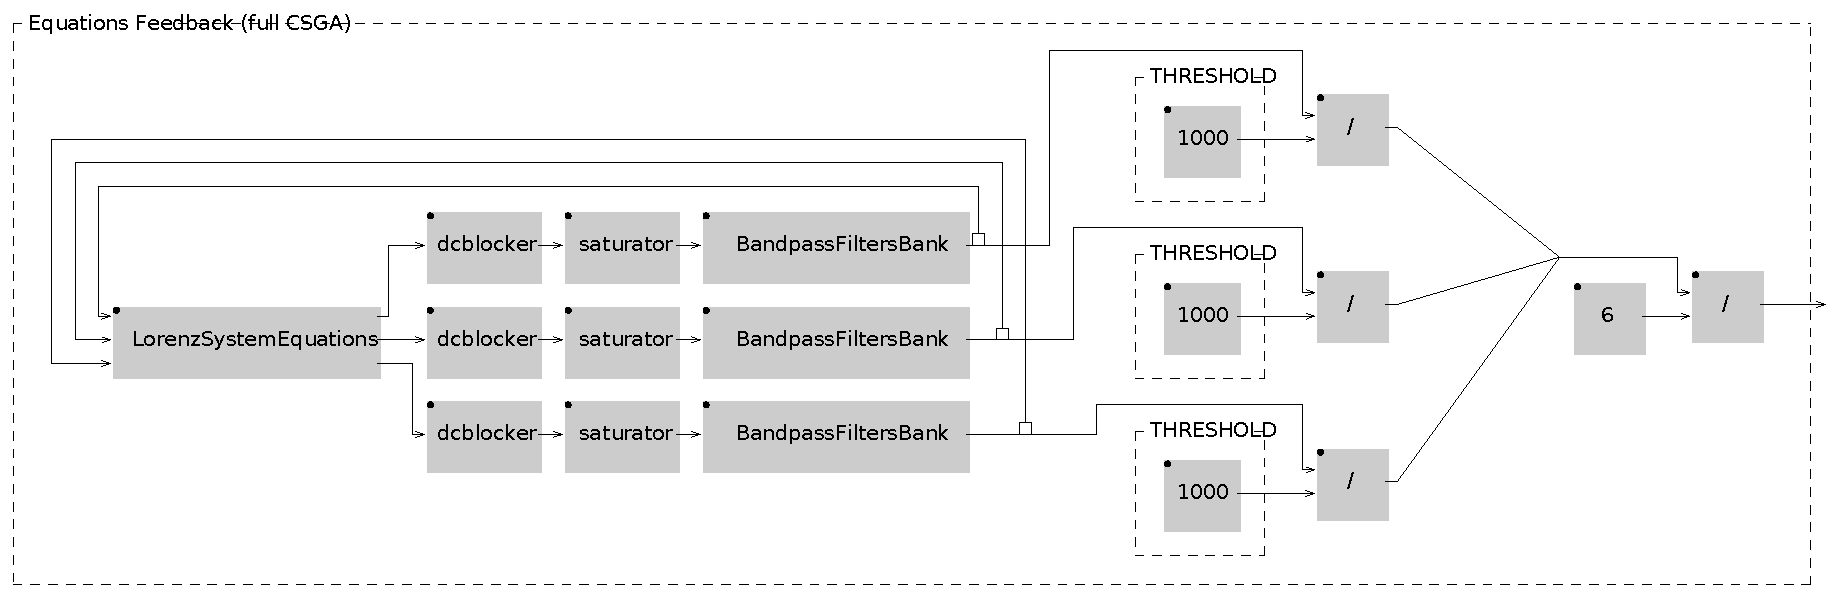
\includegraphics[width=14cm]{figures/LorenzSystemFB3.pdf}
    \caption {Topologia del feedback delle Equazioni del Sistema di Lorenz Modificato con Filterbank}
\end{center}
\vspace{0.5cm}
\end{figure}

\clearpage
\begin{figure}[h!]
\begin{center}
    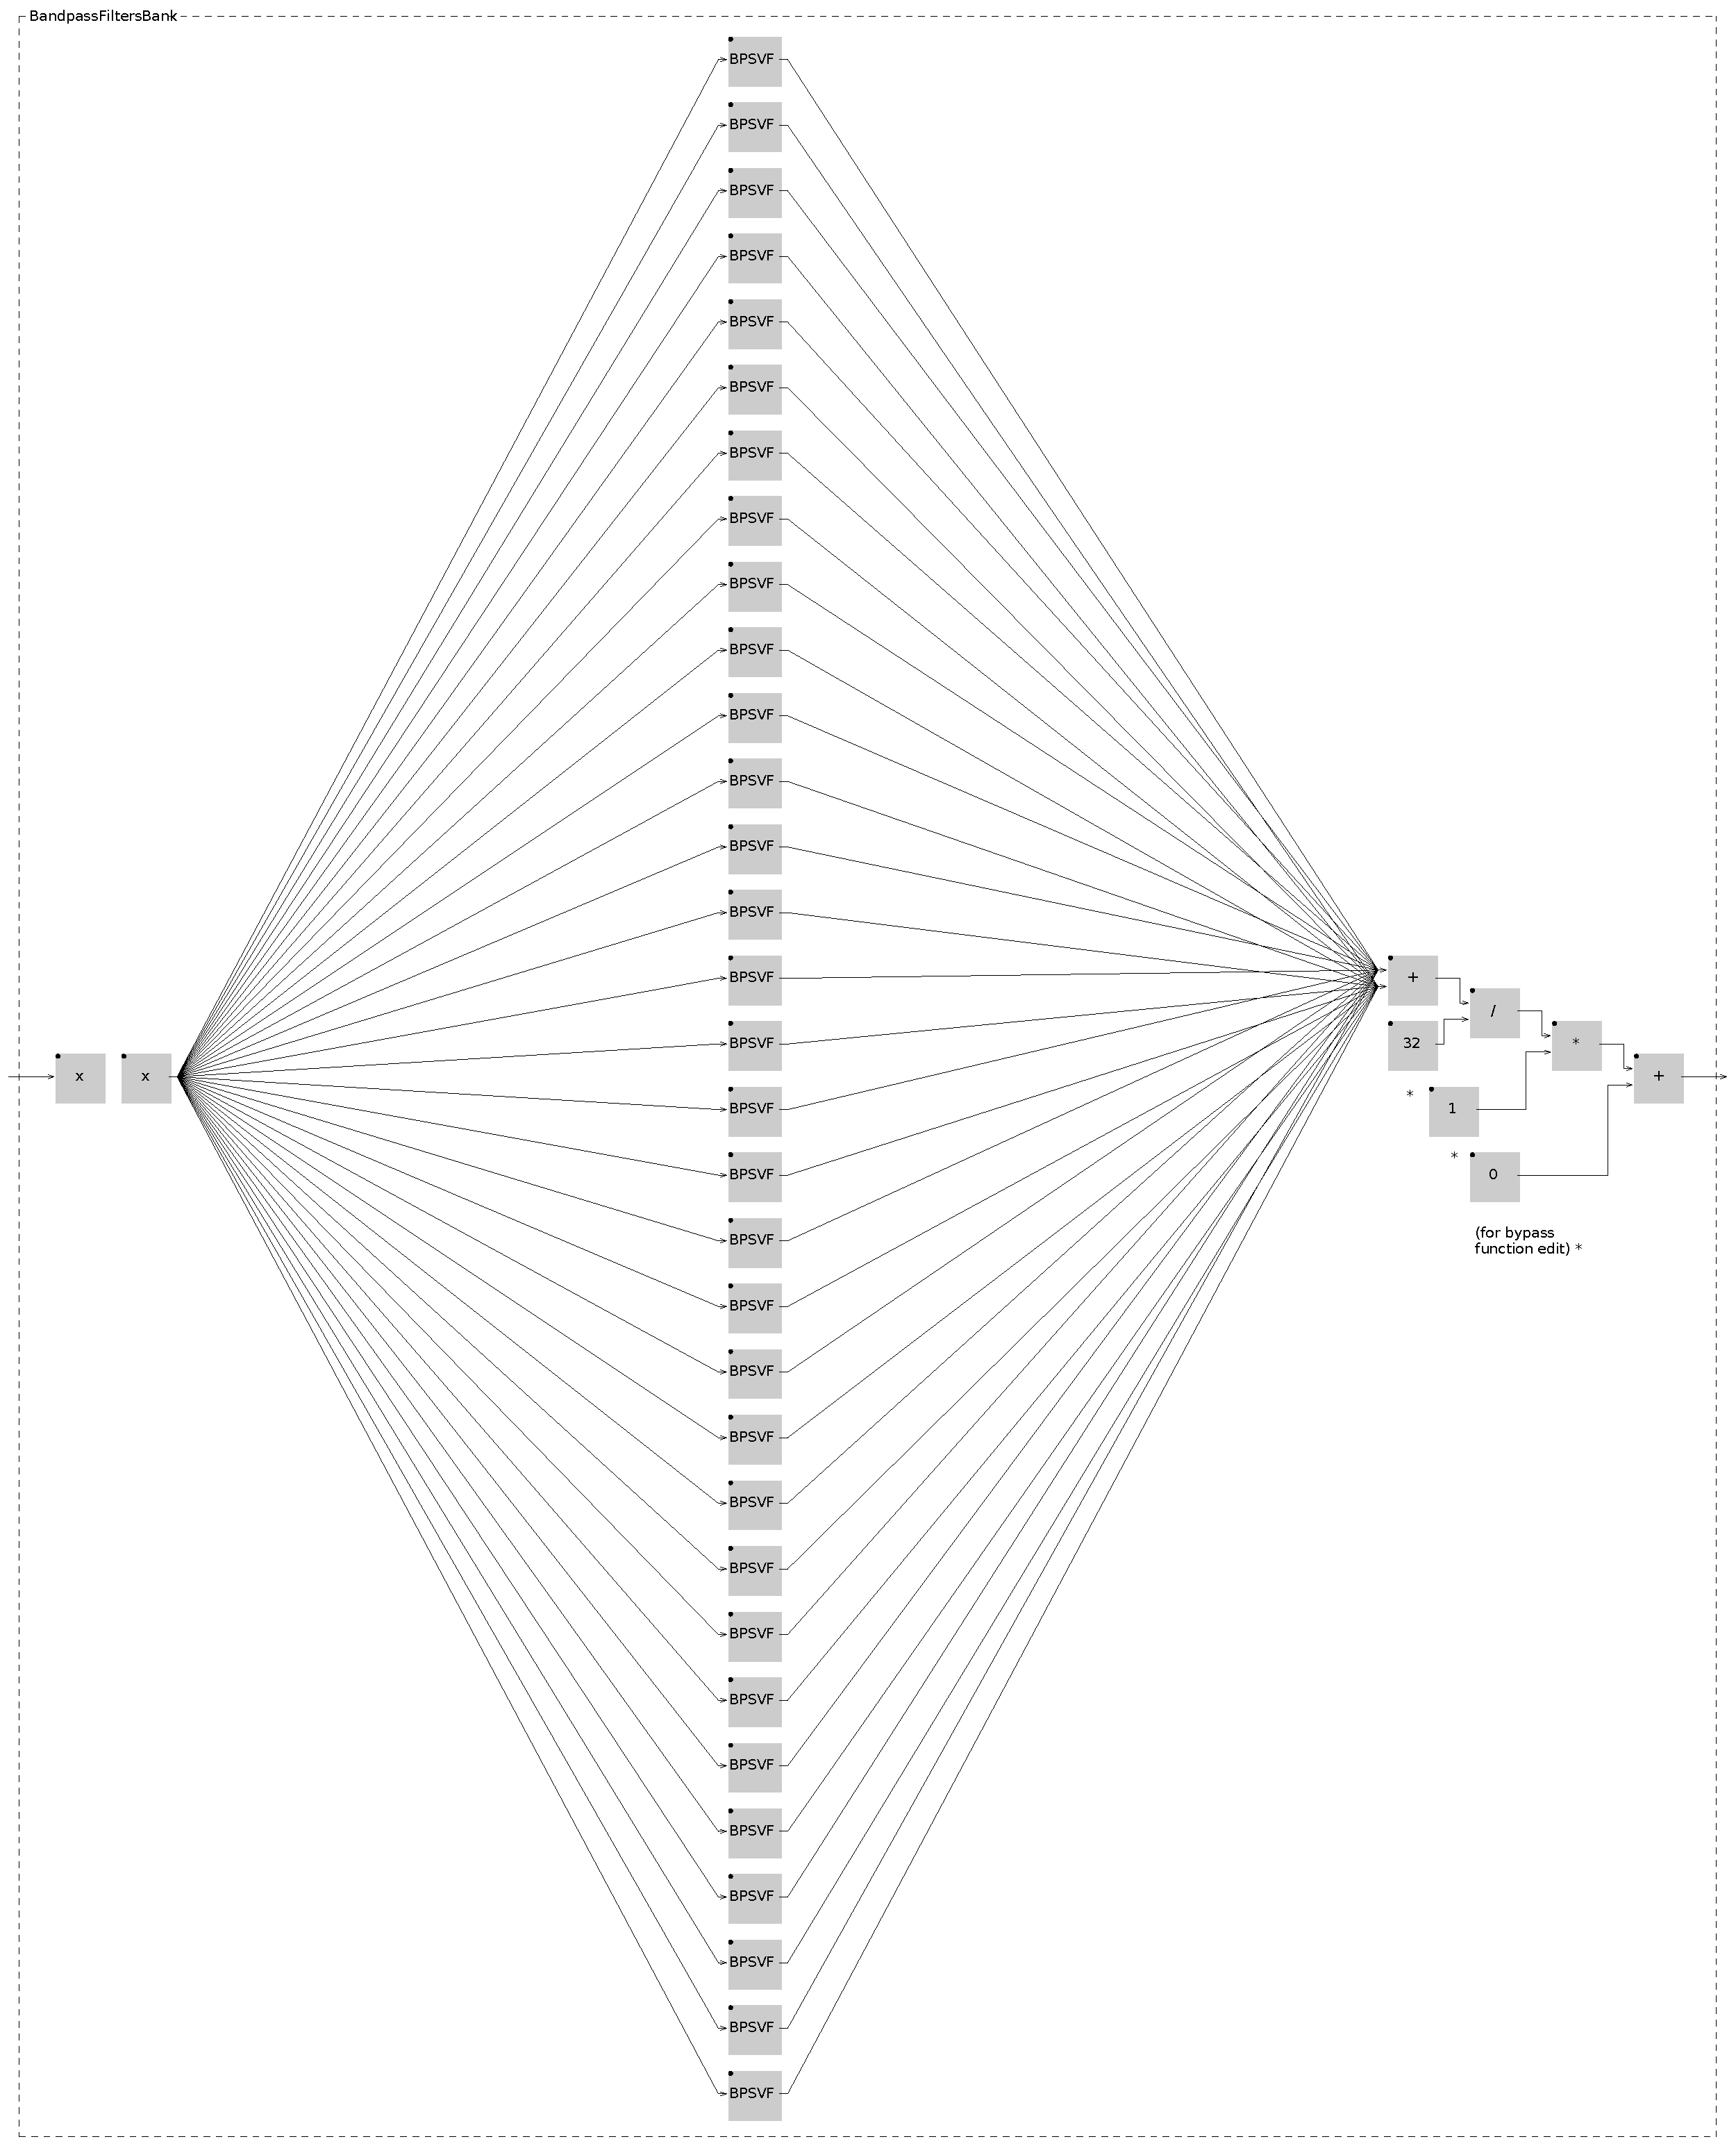
\includegraphics[width=15cm]{figures/BPFilterBank.pdf}
    \caption{Topologia del Filterbank con i filtri Bandpass SVF TPT}
\end{center}
\vspace{0.5cm}
\end{figure}

Questo andrà a rappresentare un singolo Agente richiamato all'interno della FDN.
Prima di passare alla descrizione globale della rete,
voglio ringraziare qui Edoardo Staffa per avermi assistito 
nel realizzare un semplice metodo di analisi DFT per i file audio .wav 
tramite alcune librerie nel Linguaggio di programmazione Python3.
In un secondo momento ho poi modificato il codice per 
ottenere le liste con il metodo che mi occorreva per informare i filtri di Faust.
L'algoritmo in Python è il seguente:

\vspace{0.5cm} 
\lstinputlisting[breaklines, frame=trBL, caption={Algoritmo della DFT in Python}]
{codes/DFT.py}

Questo codice prende come argomenti:
un file audio .wav in ingresso, 
un range compreso fra una frequenza minima e massima, 
il numero di bin da utilizzare per l'analisi DFT,
ed infine il numero di picchi ordinati per frequenze dalle più alte in ampiezza
che si vogliono in output con i relativi valori di ampiezze, 
con il bandwidth dell'analisi.
E in queste liste in output: frequenze, ampiezze e bandwidth,
i valori di frequenza in uscita dall'analisi simili a quelli già salvati 
in un intervallo di 40Hz, vengono eliminati, 
e i restanti picchi principali salvati nel file .lib

\subsection{Feedback Networks}
\label{Feedback Networks}

Per concludere questa osservazione sulla struttura sistemica di RITI,
discuterò brevemente, ripetendo alcuni concetti fondamentali illustrati ad inzio capitolo.
I tre stati di feedback principale su cui si basa questo sistema sono:
Il feedback interno alle equazioni differenziali, o chiamato anche come fattore di magnificazione; 
ne possiamo vedere un implementazione in questo paper\footcite{liang_difference_2013}.
Questo ci permette di poter portare le equazioni di Lorenz da uno stato di autoscillazione al
solo funzionamento come funzione di trasferimento (waveshaping) per il segnale in ingresso.
Il feedback della FDN, permette ai segnali presenti nella rete di ricircolare
con opportuni tempi di ritardo, così da avere delle decorrelazioni fra i CSGA, oltre che dei comportamenti del sistema
che possano avere una loro storia nel tempo, anche nel tornare quando il fattore di magnificazione di Lorenz è pari a 0
così da poter apprezzare solo la storia del sistema all'interno della rete senza avere nuovi contributi.
Ed infine, poiché ho dotato le equazioni di Lorenz di un ingresso esterno che viene sfruttato
sia dalla reiniezione dei segnali provenienti dalla FDN, che dall'aggiunta di 4 microfoni esterni,
il sistema viene aperto all'ambiente: perturbato dagli stessi segnali che produce all'interno della stanza,
che ne variano il comportamento nel tempo, e da fenomeni di Larsen che emergono quando il fattore di 
magnificazione che produce l'autoscillazione in Lorenz ha un contributo energeticamente 
inferiore rispetto a quello del Larsen proveniente dalla stanza.
\clearpage

\begin{figure}[h!]
\begin{center}
    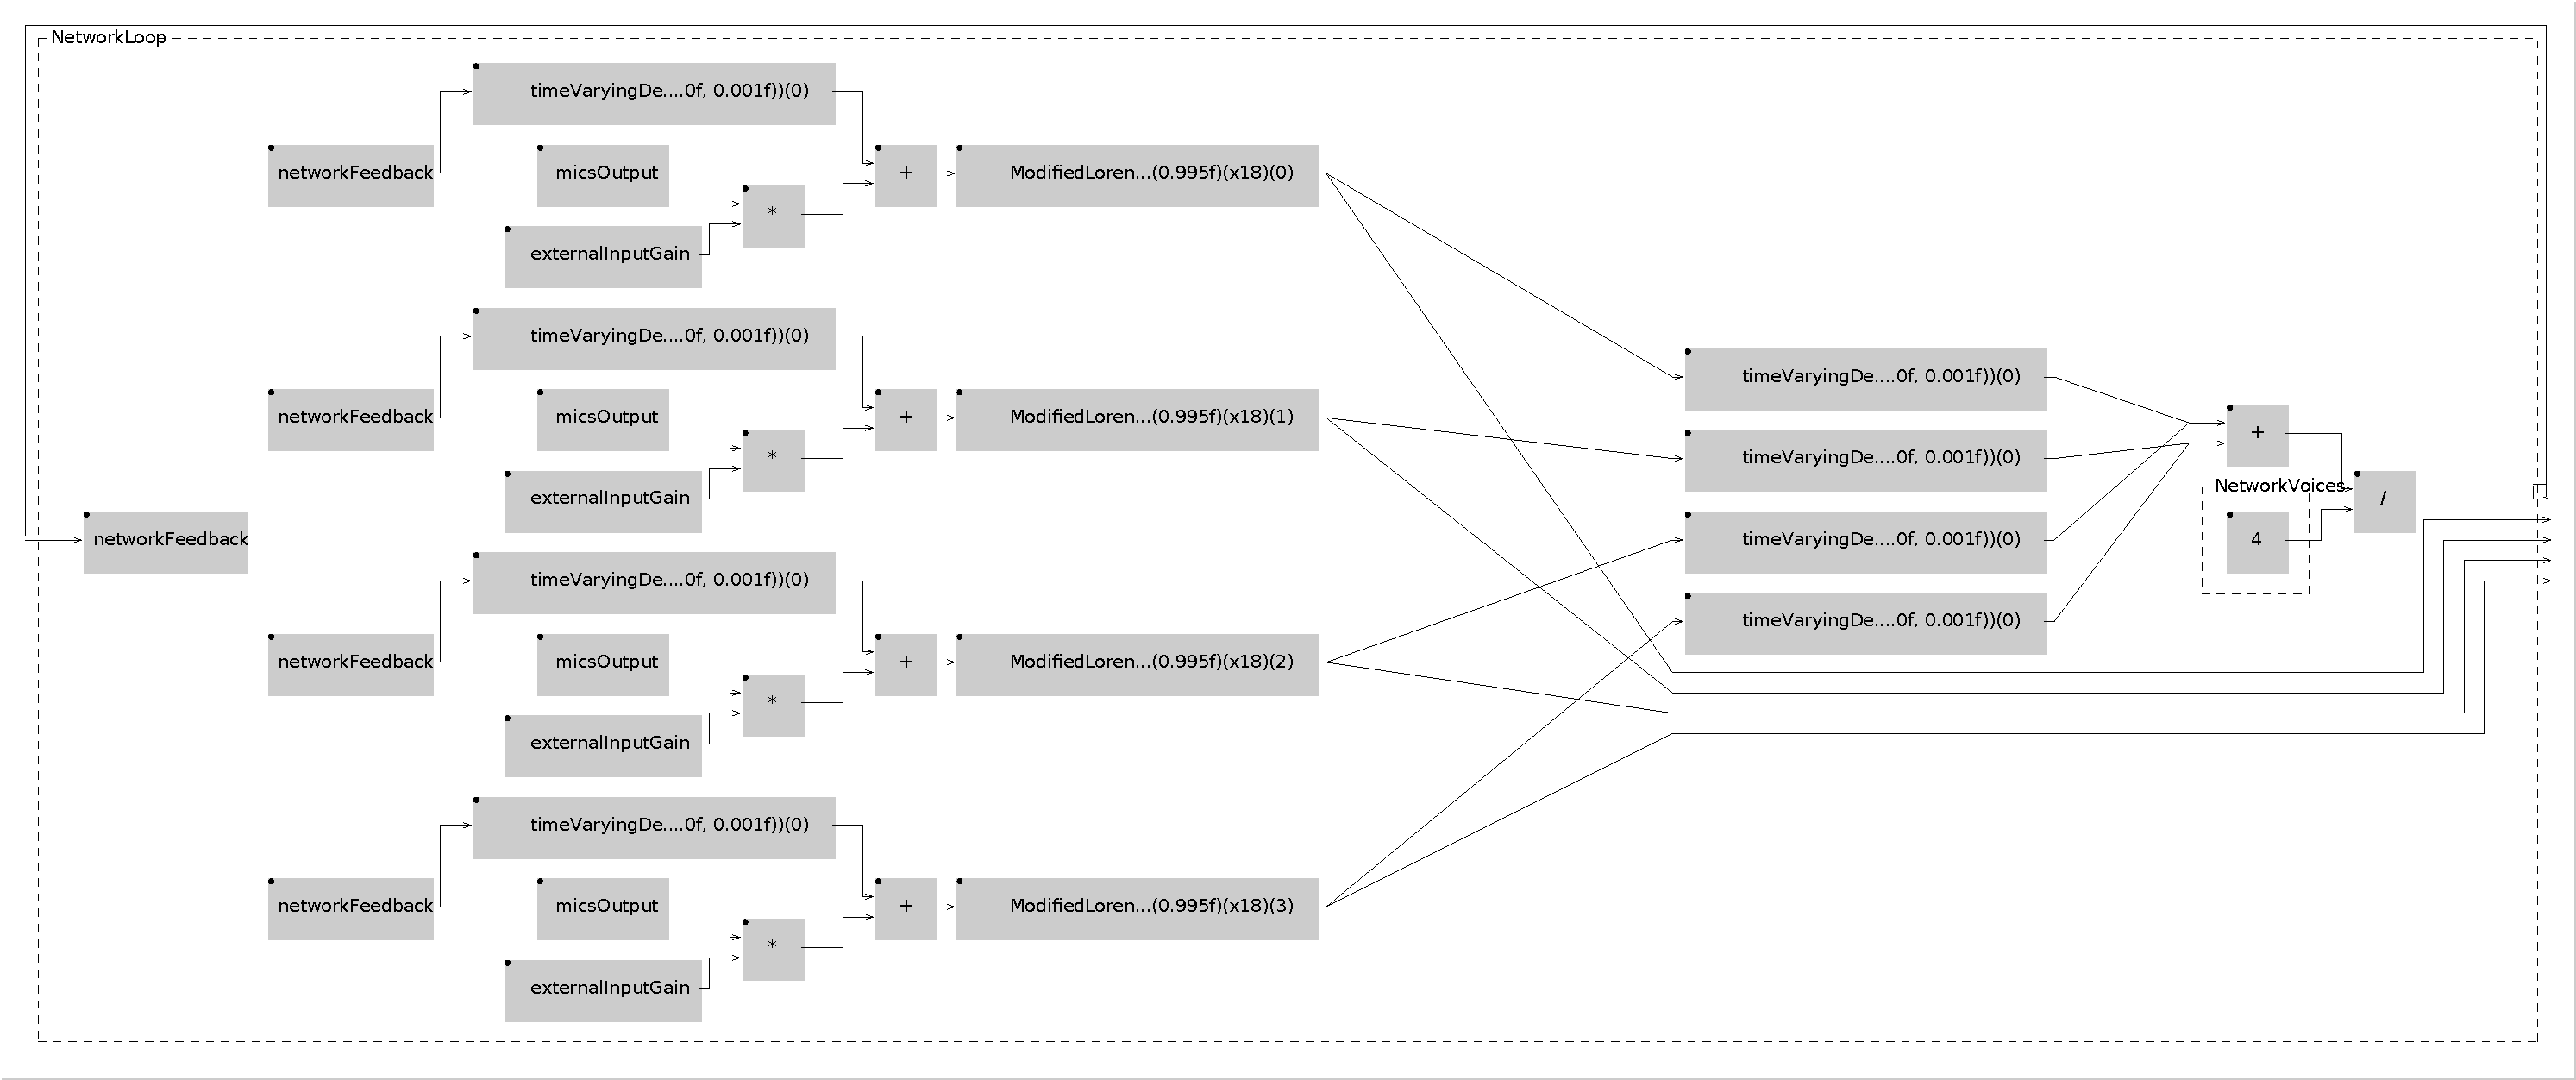
\includegraphics[width=15cm]{figures/RITI4VoiceNetwork.pdf} \\
    \caption {Esempio della Rete di RITI compilata con 4 Voci (4 CSGA)}
\end{center}
\end{figure}

\vspace{0.5cm}

La possibilità di regolare i tre stati di feedback e di portare il sistema "sulla soglia del caos"
esplorando nella performance tutti i suoi spazi, 
rivolgendo gli altoparlanti verso le pareti trasformando così l'ambiente stesso
nello spazio di sistema, rappresenta per me un estensione: del concetto di strumento musicale, 
dell'interazione con la macchina, ed infine dell'utopia di un nuovo ascolto,
in un mondo dove è sempre più necessario prendere consapevolezza della complessità che ci circonda.

\subsection{Motivazioni Personali}
\label{Motivazioni Personali}

Prima di concludere questo elaborato, 
vorrei prima soffermarmi a spiegare alcune delle motivazioni 
personali che hanno suscitato in me l'interesse per i 
sistemi complessi adattivi in live electronics, 
e che mi hanno spinto in particolare alla creazione di questo brano. \\
In questi ultimi anni di studi musicali, sono emerse nel mio fare musica 
delle questioni per me di fondamentale importanza che hanno accompagnato il mio operato
e che hanno mosso il mio interesse verso i le cibernetiche in musica. \\
In primo luogo indagare rispetto al rapporto che esiste fra l'interprete, la notazione, e lo strumento musicale;
che può essere vista in qualche modo come una parte contenuta all'interno 
della relazione fra uomo-macchina-ambiente di cui parla
Agostino Di Scipio. \\
Le prime forme di semiografia musicale possono essere rintracciate in diverse civiltà 
che risalgono addirittura attorno al 2000 A.C.,
sin d'allora l'uomo ha posto al centro della sua indagine l'interrogativo sul come fissare sempre meglio 
successioni strutturate di suoni semplici o complessi tramite una serie di parametri nel dominio discreto (la notazione), 
e che interpretati in un secondo momento potessero restituire l'idea iniziale in una resa 
acustica nel dominio del continuum temporale.
Questi parametri principalmente impiegati nella semiografia musicale Occidentale, 
sono stati fino all'incirca ad inizio del XX Secolo: 
le altezze dei suoni, le intensità, i ritmi, le durate, ed infine il timbro desiderato, 
quest'ultimo descritto richiedendo l'impiego di un certo strumento musicale o di specifici gruppi strumentali.
Tuttavia il significato stesso del termine musica non è comunque univoco ed ha avuto (ed ha ancora ad oggi) 
diverse accezioni utilizzate nei vari periodi storici.
Difatti con l'arrivo del XXI Secolo, sono state messe in crisi le nozioni di strumento musicale e di semiografia musicale, 
in quanto la pratica del comporre non si è più solamente limitata al comporre 
con i timbri dei diversi strumenti musicali, ma si è aperta anche alla possibilità del comporre stesso nel timbro, 
spingendo i compositori a cercare vie alternative ed alle volte individuali in cui scrivere musica differente dalla tradizione.\\
Riguardo gli strumenti musicali invece, se la voce è difatti il primo strumento dell'uomo in quanto 
abita il corpo stesso che ne è il custode, la macchina che nel suo senso generico è qualsiasi strumento 
il cui moto relativo trasmetta o anche amplifichi la forza umana.
Sin dall'antichità la macchina si è prestata all'impiego come strumento musicale sottoforma di qualcosa per assistere l'uomo nella 
sua intenzione del fare musica secondo l'organizzazione dei parametri esposti precedentemente; 
con la composizione nel timbro viene invece a mancare l'idea 
di una musica composta solamente da queste tipiche relazioni tramite gli strumenti musicali, 
rivalutando l'idea stessa che si ha di uno strumento musicale, aperta ora di fatto alla possibilità 
del poter comporre quanto il timbro stesso integrando anche la creazione dello strumento che lo produce. \\
Come dice Trevor Wishart nel suo libro On Sonic Art:

\begin{center}
    \vspace{0.5cm}
    \textit{In this book i will suggest that the logic of this assertion is inverted.
    It is notability which determines the importances of pitch, rythm, and duration and
    not vice versa and that much can be learned by looking at 
    musical cultures without a system of notation... 
    In this book, I will suggest that we do not need to deal with a finite set of
    possibilities. The idea that music has to be built upon  finite lattice and the
    related idea that permutational procedures are a valid way to proceed will
    be criticised here and a musical methodology developed for dealing with a
    continuum using the concept of transformation}\footcite{wishart_on_sonic_art}
\vspace{0.5cm}
\end{center}

Come comportarsi quindi davanti ad una condizione in cui viene messa in crisi l'idea stessa
che si ha di musica, di notazione musicale, e di strumento musicale?\\
Questa indagine mi ha portato a rivolgere l'attenzione al rapporto con la notazione 
e gli strumenti musicali in quelle opere dei compositori contemporanei, 
che raccogliendo le ceneri di questa crisi del XXI Secolo, 
hanno deciso di approfondire l'idea dietro l'utilizzo
di uno strumento musicale con cui fare musica, non più come 
qualcosa di funzionale al riprodurre dei parametri annotati in partitura a priori,
ma come un sistema che offre una serie di possibilità; 
in cui lo strumento diviene il corpo acustico su cui indagare 
tutta una serie di relazioni e gesti possibili dell'interprete, 
alla ricerca di un'esplorazione sonora dello spazio del sistema,
e in cui la partitura diviene traccia del come replicare l'esistenza di 
qualsiasi tipo d'interazione con il sistema.
In tal senso Trevor Wishart suggerisce di guardare alla Teoria delle Catastrofi 
di René Thom, assumendo che le regole formali di una musica passono
essere ricavate dall'osservazione di uno strumento stesso come se questo fosse un sistema.
Nella mia indagine per portare dei validi esempi, ho dunque rintracciato questo tipo di atteggiamento 
nei confronti dello strumento
e della notazione in alcune opere come: Pression di Helmut Lachenmann,
dove la partitura viene ad indicare come agire sul corpo dello strumento
schiudendone nella sua totalità il suo mondo sonoro accessibile,
o nell'opera Necessità d'interrogare il cielo di Giorgio Netti,
dove a partire dagli elementi della notazione tradizionale, lo studio condotto 
sul corpo dello strumento e degli esiti acustici del gesto, scendono così tanto 
"ad un basso livello di articolazione" da schiuderne in questo tutta una serie di nuove possibilità
acustiche, o anche nei lavori stessi di Wishart, come nel ciclo Vox 
dove la voce viene esplorata in tutte le sue ambiguità rendendo
complesso il collegamento fra il suono e la sorgente che lo produce. \\
In senso più generale la storia della musica elettroacustica è fortunatamente costellata 
di pionieri che hanno messo in crisi il linguaggio musicale e l'impiego degli strumenti musicali,
ma l'ulteriore scarto che propongo qui, consiste nel fatto che se è vero quindi come 
dice Trevor Wishart che le regole formali di una musica possono
essere ricavate dall'osservazione di un sistema, 
la pratica del disegnare un sistema autonomo (la macchina) con cui fare musica,
ne riflette di conseguenza la quantità di informazione che questo contiene al suo interno,
e di conseguenza il tipo di relazioni e interazioni con il suo ambiente che 
ci interessano dal punto di vista compositivo.\\
In secondo luogo, ho trovato interessante indagare rispetto al rapporto conflittuale che l'uomo ha con la tecnologia
nella società contemporanea. 
In effetti, l'uomo ha da sempre un rapporto conflittuale con la tecnologia,
se sin dai tempi di Platone emergevano queste problematiche e preoccupazioni
relative alla discretizzazione del pensiero con la scrittura
(come possiamo leggere in Fedro), 
giungendo alle paure più attuali di Norbert Weiner di fronte
alla scoperta della cibernetica, possiamo dire che la sua paura di una società contemporanea 
composta da interazioni sistemiche fra l'uomo e la macchina
in cui il primo è succube della seconda, sembra in qualche modo essere stata profetica ed essersi realizzata.
Come scrive Norbert Wiener nel suo libro Introduzione alla cibernetica. L'uso umano degli esseri umani,
inizialmente pubblicato con il titolo The Human Use Of Human Beings: Cybernetics And Society\footcite{wiener_introduzione_nodate}
nel 1950:

\begin{center}
    \vspace{0.5cm}
    \textit{La nostra concezione della società ideale differisce dalla società ideale
    prospettata dai fascisti e da molti magnati del mondo degli affari 
    e della politica.
    Essi preferiscono una organizzazione in cui tutti i comandi
    provengano dall'alto senza che sia possibile nessuna riverisbilità.
    Sotto di essi gli uomini sono stati ridotti al livello di esecutori degli ordini
    di un centro nervoso che pretende di essere superiore.
    Desidero che questo libro sia inteso come una protesta contro questa
    utilizzazione inumana degli esseri umani, poiché sono convinto che impiegare
    un uomo richiedendogli e attribuendogli meno di quanto comporta la sua condizione umana,
    significa abbruttire questa condizione e sperperare le sue energie.
    È una degradazione della condizione umana legare un uomo a un remo e impiegarlo come
    sorgente di energia; ma è altrettanto degradante segregarlo in una fabbrica
    e assegnarlo a un compito meramente meccanico che richieda meno di un milionesimo
    delle sue facoltà cerebrali. È assai più facile infatti
    organizzare una fabbrica o una galera che impieghi gli esseri umani
    per una insignificante frazione delle loro attitudini che costruire una 
    società in cui essi possano elevarsi in tutta la loro statura.
    Coloro che soffrono di un complesso di potenza sanno che la meccanizzazione 
    dell'uomo è il mezzo più semplice per realizzare le loro ambizioni.
    Sono convinto che questa facile via al potere comporta non soltato l'annullamento 
    di quelli che io credo siano i valori morali dell'umanità,
    ma anche l'eliminazione delle attuali, labilissime possibilità di
    sopravvivenza della razza umana per un periodo considerevole.
    }
\vspace{0.5cm}
\end{center}

Se in risposta a questa affermazione di Wiener passiamo ad una seconda citazione, proveniente invece da un libro 
recente che critica la nostra condizione nella società contemporanea, scritto e pubblicato da François J. Bonnet. nel 2020:

\begin{center}
    \vspace{0.5cm}
    \textit{The increasingly frenetic accumulation of sounds and
images is a part of this intensification, aiming to fill the void of
a present that is forever sinking into the past. At every
moment, the world must be supplied with novel sensory
material generated to replace existing material that has
already become obsolete. The exaltation of the present as the
promise of pleasure Is therefore never really meant to be actualised,
since it will immediately be obsolesced by a continuously
renewed influx of promises.
Needs, cravings, and desires
are endlessly rebooted.
The present moment, as constructed by our society, is
nothing but a procedure of forgetting, a catalyst for amnesia,
and as such it enables the repetition which, in turn, through
the presentation of novelty, allows us to distance ourselves
3 little further from the past. And this writing and rewriting
of the present—as if it were a palimpsest—continues to
accelerate, demanding that we forget at an ever higher fre-
quency. What was is of no concern; all has beens are eliminated
in favour of what is, with little regard for what will be.
Where the modern era anticipated a present yet to come,
transposing current momentum into future accomplishments,
our postindustrial, postmodern era sees the future as
nothing but a vague, indeterminate site hosting an indistinct
cloud of promises and signs as desirable as they are deadly.}\footcite{francois_jbonnet_after_death}
\vspace{0.5cm}
\end{center}

Troveremo che non solo le paure profetiche di Wiener si sono realizzate già da diverso tempo, 
ma che da molto tempo ne stiamo già raccogliendo le inevitabili conseguenze,
che si riflettono dal mio punto di vista in una società anestetizzata, 
schiava della tecnologia, e livellata in qualche modo ad una condizione di eterno presente.
In risposta a questa condizione, disegnare i propri sistemi e di conseguenza riappropriarsi della tecnologia,
rappresenta per me un modo costruttivista di rispondere ai problemi del mondo contemporaneo
attraverso la pratica musicale.\\
Per concludere infine le motivazioni che mi hanno portato a questo tipo di scrittura musicale, 
l'ultimo aspetto che ho reputato importante affrontare è la forma,
nei suoi aspetti Macro-temporali e Micro-temporali. \\
Se ammettiamo quindi come sostiene François J. Bonnet, ed altri filosofi come Mark Fisher e Slavoj Žižek,
che la nostra società contemporanea ha in qualche modo normalizzato
una velocità schizofrenica nelle cose, dove tutto deve essere estremamente funzionale per motivi pratici,
e dove non abbiamo più modo di esercitare alcun controllo sullo scorrere del tempo,
la riappropriazione del tempo nella forma, dell'ascolto, ed infine dello spazio, diviene per me un elemento fondamentale
nella composizione,
dove tutti gli elementi del sistema hanno un ruolo condiviso che contribuisce 
a formare la complessità nel suo insieme.
A tal proposito ho sempre trovato interessante osservare nelle evoluzioni temporali 
come un piccolo cambiamento all'interno di un sistema possa conseguentemente portare 
a cambiamenti radicali
nella Macroforma; proprio come nella sensibilità alle condizioni della teoria del caos, 
che ci illustra come in un sistema caotico, a variazioni infinitesime delle condizioni iniziali 
corrispondono variazioni significative del comportamento futuro. 
Dunque in tal senso è diventato per me un aspetto importante lavorare con
sistemi emergenti che possano rendere udibili questi processi di continua trasformazione
del suono, e che non rendano udibile una sola traiettoria possibile nell'evoluzione formale
di un brano.\\
È a tal proposito che Stockhausen, nella sua teoria della "Forma unificata del tempo", 
notò già nel 1960 come in tal senso la differenza fra i Micro-elementi nella forma, 
e la Macroforma, non consista tanto in diversi ruoli e compiti del comporre,
quanto più a diversi livelli di percezione del tempo, 
poiché altezza e ritmo sono fondamentalmente la stessa cosa se percepita a diverse scale temporali,
e ce lo illustra nella sua composizione Kontakte realizzata fra il 1958 ed il 1960, 
mettendo in certi termini in luce,
come nella forma di un brano musicale il ruolo delle parti sia sostanzialmente un problema 
di complessità
che dipende dal punto di vista dell'osservatore.

%\subsection{Conclusioni}
%\label{Conclusioni}
%
%In conclusione, 
%abbiamo avuto modo di introdurre l'argomento delle cibernetiche in Musica,
%parlando di come l'esigenza di un pensiero sistemico 
%abbia pian piano fatto breccia nell'operato
%di alcuni dei più importanti compositori del XX Secolo. 
%Arrivando fino ad osservare e studiare il realizzarsi di questa condizione
%attraverso l'operato di Dario Sanfilippo e da Agostino Di Scipio, 
%di cui abbiamo approfondito alcuni dei principali meccanismi presenti nei loro lavori compositivi,
%nel desiderio di creare attraverso questi modelli
%una strada da seguire per la composizione dei sistemi complessi adattivi per la
%performance musicale in live electronics.
%Ed Infine mettendo in luce l'importanza di una prospettiva 
%ontologica ed epistemeologica nella composizione musicale sistemica.
\clearpage 

\cleardoublepage

\appendix

\thispagestyle{empty}
\section{First appendix}

\section{Second appendix}
%% ---------------------------------------------- Bibliografia -----------------
\clearpage
\printbibliography
%% --------------------------------------------------------------------- Fine --
\end{document}